\chapter{Yoneda I: Internal vs. external}

This section marks the start of a long journey that ends in
the statement and proof of the famous Yoneda lemma in category theory (\todo).
As with any important concept in category theory, the Yoneda lemma
can be understood through a variety of perspectives. In these
notes we will explore a particular perspective that feels most
relevant to PL: the Yoneda lemma is a means of connecting
the ``internal'' to the ``external''.

Consider, for example, the case of product.
In the preceding sections, we have given you the definition of product
that is most commonly found in standard textbooks on category theory.
This definition has an ``internal'' character, because it defines
product in a category \(\calC\) purely in terms of
other objects and morphisms \emph{inside} of \(\calC\).

But there is another way to define product.
Think back to \cref{thm:calc-products},
which showed how to interpret a simple programming language
in an arbitrary category \(\calC\) with finite products.
The proof of \cref{thm:calc-products} gave a recipe
for interpreting each of the judgments of programming language
in \(\calC\). Following this recipe,
each of the typing rules became
\emph{functions on morphisms}. For example, the typing rule
\[
\inferrule*[right=T-Fst]{\Gamma \vdash M : A \pltimes B}{\Gamma \vdash \plfst{M} : A}
\]
for projecting out the first component of a pair
was interpreted as a function
\begin{align*}
  \{\text{morphisms \(\llbr\Gamma\) to \(\llbr{A\pltimes B}\)}\}
  \longrightarrow
  \{\text{morphisms \(\llbr\Gamma\) to \(\llbr{A}\)} \},
\end{align*}
namely the function
that sends interpretations of \(\llbr{M}\) to interpretations of \(\llbr{\plfst M}\).

It turns out that we can promote this recipe into a \emph{definition} for product.
In contrast to the textbook definition in terms of objects and morphisms
of \(\calC\), this definition characterizes the product in terms of \emph{functions} between
\emph{sets} of morphisms. This gives it an ``external'' character,
because it defines the product in terms of set-theoretic objects (sets and functions)
that live \emph{outside} of \(\calC\).

Of course, it will make no difference whether one chooses the internal
or the external definition of product: as we will see further down the line,
the Yoneda lemma implies that the two formulations are equivalent.
As a warm up to this abstract proof, this section will show
concretely how the equivalence works for the special case of products.

First, we must make precise what we mean by this ``external'' definition of product
that defines product in terms of functions on morphisms.
To formalize this idea of ``maps between morphisms'',
  it's useful to have the following definition that we've put off for a long time.

\begin{definition}[Hom-set]
  Let \(X\) and \(Y\) be objects of a category \(\calC\).
  The \emph{hom-set} of $\calC$ at $X$ and $Y$, 
  written \(\calC(X,Y)\),
  is the set of morphisms from \(X\) to \(Y\):
  \[
  \calC(X,Y) := \{f \mid \dom(f) = X, \cod(f) = Y\}.
  \]
\end{definition}
\marginnote{%
The word ``hom'' is an abbreviation of ``homomorphism'',
and the name hom-set comes from the fact many of the original motivating examples of categories
had morphisms that were homomorphisms between algebraic structures.
}
For example, \begin{itemize}
\item In the category of finite sets and set functions $\FinSet$, the
  hom-set $\FinSet(\{a,b\}, \{1, 2, 3\})$ is the set of all functions
  from $\{a,b\}$ to $\{1, 2, 3\}$.
\item Hom-sets can be empty. In the divisibility category $(\mathbb{N}, \preceq)$,
the hom-set $\mathbb{N}(3,4) = \emptyset$, while $\mathbb{N}(3, 6) = \{\top\}$.
\end{itemize}
This definition lets us state formally what it means for an inference rule
like \(\textsc{T-Fst}\) to denote a function from morphisms to morphisms.
We shall say that the interpretation of \(\textsc{T-Fst}\) is
a family of functions \((\mathsf{Fst}_\Gamma)_{\Gamma\in\calC}\),
indexed by the ambient context \(\Gamma\),
of the following type:
\[
\mathsf{Fst}_\Gamma : \calC(\Gamma, A \times B) \to \calC(\Gamma, A)
\]

%% Let's pause to inspect the unusual shape of this function.
%% First, observe that this is a function between two sets: this is \emph{not} a
%% morphism in the category $\calC$.  Second, it is a function between two sets of
%% morphisms with the same domain, $\Gamma$.  And third, the function is
%% \emph{indexed by $\Gamma$}, written with a subscript. We can visualize elements
%% of this family of ``$\mathsf{Fst}$-like morphisms'' as follows:
We can visualize this family of functions as follows:
\begin{equation}
  % https://tikzcd.yichuanshen.de/#N4Igdg9gJgpgziAXAbVABwnAlgFyxMJZABgBpiBdUkANwEMAbAVxiRAB12BxOgW17oB9AIwgAvqXSZc+QijLCqtRizace-IQCZxkkBmx4CRMlqX1mrRB258BggMy6ph2UWGlF1C6usBBAAJOPF54AIAhAOd9aSM5ZC1SM28VKxA-aIMZY3lSB3NUtgA6EvElGCgAc3giUAAzACcIXiQyEBwIJAcUyzZKkRBqBjoAIxgGAAVYt2ssMGxYaMbm1uoOpAAWajGwKC62nzS6gaHR8anXHJA5hdYJeqaWxA92zsRu5V7rfp1TscnplcblhFvcQMsni91ogtp9fODBL8QMN-hdsnJrvMQXc9BCkIlXl0evD+k4-udARjgaDcY98Ws3rCURTLlSsYtiUdHGUxEA
\begin{tikzcd}
  {\color{red} \Gamma_1} \arrow[rd, "f" description, color = red] \arrow[rrdd, "f'" description, bend left, color = red] &             &   \\
  {\color{blue}\Gamma_2} \arrow[r, "g" description, color = blue] \arrow[rrd, "g'" description, color = blue]              & A \times B  &   \\
  {\color{orange} \Gamma_3} \arrow[ru, "h" description, color = orange] \arrow[rr, "h'" description, color = orange]              &             & A \\
  ...                                                                               &             &  
  \end{tikzcd}
  \label{cd:indexed-fam}
\end{equation}
As an example of working with this function, we have that
$\mathsf{Fst}_{\Gamma_1}(f) = f'$.

In addition to the basic type shown above, we will also require that \(\mathsf{Fst}\)
be \emph{natural} in \(\Gamma\).
Intuitively, what this means is that \(\mathsf{Fst}\) is in a sense ``polymorphic in \(\Gamma\)''.
Just as polymorphic functions in System F
respect ``change of representation'' for the type variables that they are polymorphic over~\citep{reynolds1983types},
we will require that the family of functions \((\mathsf{Fst}_\Gamma)_{\Gamma\in\mathsf{Ob}(\calC)}\)
respect ``change of \(\Gamma\)''.
Concretely, this means that if any input \(f\) as shown in the pictue above is changed into \(f \circ s\) via some morphism
$s : \Gamma' \to \Gamma$,
it must be the case that \(\mathsf{Fst}_\Gamma(f)\) is changed into \(\mathsf{Fst}_{\Gamma'}(f\circ s)\)
via \(s\) too. Formally, the following \emph{naturality condition} must hold for any such \(f\) and \(s\):\marginnote{We will save a formal abstract definition
of naturality for \todo.}

%% There may be many morphisms that satisfy the type signature of $\mathsf{Fst}$,
%% but the key is that there are relatively few that are
%% \emph{invariant under the choice of $\Gamma$}. Concretely, if
%% there are is a morphism $s : \Gamma' \to \Gamma$ that relates $\Gamma'$ to $\Gamma$,

%% We will build towards the idea that there is some family of ``\textsf{Fst}-like
%% functions'' that ought to behave coherently for different choices of context
%% $\Gamma$.  The notion of coherence we need is stability under parallel substitution.

\begin{align*}
  \mathsf{Fst}_\Gamma(f) \circ s = \mathsf{Fst}_{\Gamma'}(f \circ s)
\end{align*}
Another intution for this condition comes from the requirement that the interpretation of a programming language
be \emph{stable under substitution}.
For instance, we know that
$\plfst{M}$ is invariant under substitution for some (possibly multi-way)
substitution $s$:
\begin{align*}
  (\plfst{M})[s] \equiv \plfst{(M[s])}
\end{align*}
This program equation corresponds directly to the naturality condition given above.

Applying the above analysis to the typing rule \textsc{T-Snd}
gives an analogous function for extracting the second component of a pair:
\begin{align*}
  &\inferrule
    {\Gamma \vdash M : A \pltimes B}
    {\Gamma \vdash \plsnd{M} : B}
    \rightsquigarrow
    \mathsf{Snd}_\Gamma : \calC(\Gamma, A \times B) \to \calC(\Gamma, B)
    \\
  &\text{such that }\forall s : \Gamma' \to \Gamma,
    \mathsf{Snd}_\Gamma(f)\circ s = \mathsf{Snd}_\Gamma(f \circ s)
\end{align*}
The rule \textsc{T-Pair} for forming pairs becomes a function
that takes in two morphisms and bundles them together into a morphism into the product:
\begin{align*}
  &\inferrule
    {\Gamma \vdash M : A \quad
      \Gamma \vdash N : B }
    {\Gamma \vdash \plpair{M}{N} : A \times B}
    \rightsquigarrow
    \mathsf{Pair}_\Gamma : \calC(\Gamma, A) \times \calC(\Gamma, B) 
    \to \calC(\Gamma, A \times B)
\\
   &\text{such that }\forall s : \Gamma' \to \Gamma,
    \mathsf{Pair}_\Gamma(f, g)\circ s = \mathsf{Pair}_\Gamma(f \circ s, g \circ s)
\end{align*}
Finally, the $\beta$ and $\eta$ laws become equations between nested applications of the functinos \(\mathsf{Fst}\), \(\mathsf{Snd}\),
and \(\mathsf{Pair}\).
\begin{align*}
  \inferrule
    {\Gamma \vdash M : A \quad
      \Gamma \vdash N : B }
    {\Gamma \vdash \plfst{\plpair{M}{N}} \equiv M}
    &\quad\rightsquigarrow\quad
    \mathsf{Fst}_\Gamma(\mathsf{Pair}_\Gamma(f,g)) = f
\\
  \inferrule
    {\Gamma \vdash M : A \quad
      \Gamma \vdash N : B }
    {\Gamma \vdash \plsnd{\plpair{M}{N}} \equiv N}
    &\quad\rightsquigarrow\quad
    \mathsf{Snd}_\Gamma(\mathsf{Pair}_\Gamma(f,g)) = g
\\
  \inferrule
    {\Gamma \vdash M : A \times B}
    {\Gamma \vdash M \equiv \plpair{\plfst{M}}{\plsnd{M}} \equiv N}
    &\quad\rightsquigarrow\quad
    \mathsf{Pair}_\Gamma(\mathsf{Fst}_\Gamma(f), \mathsf{Snd}_\Gamma(f)) = f
\end{align*}
Packaging up all of these constraints into a definition,\footnote{We have chosen to name this concept ``PL-product'' as it was derived from the typing rules for product types in a programming language.}
\begin{definition}[PL-product]
  \sloppy
  Let \(A\) and \(B\) be objects of a category \(\calC\).
  A \emph{PL-product} of \(A\) and \(B\) consists of:
  \begin{itemize}
  \item An object \(A \times B\)
  \item $\calC$-indexed functions:
    \begin{align*}
      \mathsf{Fst}_\Gamma &: \calC(\Gamma,A\times B) \to \calC(\Gamma,A) \\
      \mathsf{Snd}_\Gamma &: \calC(\Gamma,A\times B) \to \calC(\Gamma,B) \\
      \mathsf{Pair}_\Gamma &: \calC(\Gamma,A)\times\calC(\Gamma,B) \to \calC(\Gamma,A\times B)
    \end{align*}
  \end{itemize}
  satisfying the necessary properties to be $\calC$-indexed, i.e.:
  \begin{itemize}
  \item \(\mathsf{Fst}\), \(\mathsf{Snd}\), and \(\mathsf{Pair}\) ``respect substitution'': for all
    \(\Gamma'\xrightarrow{s}\Gamma\),
    \begin{align*}
      \mathsf{Fst}_{\Gamma}(f)\circ s &= \mathsf{Fst}_{\Gamma'}(f \circ s) & \text{for all \(\Gamma\xrightarrow{f} A \times B\)} \\
      \mathsf{Snd}_{\Gamma}(f)\circ s &= \mathsf{Snd}_{\Gamma'}(f \circ s) & \text{for all \(\Gamma\xrightarrow{f} A \times B\)} \\
      \mathsf{Pair}_{\Gamma}(f,g)\circ s &= \mathsf{Pair}_{\Gamma'}(f \circ s,g\circ s) & \text{for all \(\Gamma\xrightarrow{f} A\) and \(\Gamma\xrightarrow{g} B\)}
    \end{align*}
  \item Analogs of the \(\beta\) and \(\eta\) laws hold:
    \begin{align*}
      \mathsf{Fst}_{\Gamma}(\mathsf{Pair}_{\Gamma}(f,g)) &= f   & \text{for all \(\Gamma\xrightarrow{f} A\) and \(\Gamma\xrightarrow{g} B\)} \\
      \mathsf{Snd}_{\Gamma}(\mathsf{Pair}_{\Gamma}(f,g)) &= g   & \text{for all \(\Gamma\xrightarrow{f} A\) and \(\Gamma\xrightarrow{g} B\)} \\
      \mathsf{Pair}_\Gamma(\mathsf{Fst}_\Gamma(f),\mathsf{Snd}_\Gamma(f)) &= f   & \text{for all \(\Gamma\xrightarrow{f} A\times B\)}
    \end{align*}
  \end{itemize}
\end{definition}
Now we can state an important theorem.
\begin{theorem}
  PL-products are equivalent to ordinary products.
\end{theorem}
This theorem breaks down into multiple components.
\begin{enumerate}
\item Every PL-product can be turned into a categorical product.
\item Every categorical product can be turned into a PL product.
\item Constructions (1) and (2) round-trip to the identity.
\end{enumerate}
The proof tackles each piece separately.
\begin{construction} \label{cons:pl-prod-to-prod}
Every PL product of $A$ and $B$
can be turned into a categorical product.\footnote{In general, we will use the word ``'construction'' to signal a lemma whose proof details are going to be relevant later. In this case, we will need the precise definition of how PL products are turned into categorical ones later on, to prove that the two constructions we have done round-trip to the identity.}
\end{construction}
\begin{proof}
  Suppose you have $(A \times B, \mathsf{Fst}_\Gamma, \mathsf{Snd}_\Gamma, 
  \mathsf{Pair}_\Gamma)$. Remember, $\mathsf{Fst}_\Gamma$ (and all these 
  other functions) behave like polymorphic functions, and we 
  need to find a diagram like:
  \begin{center}
   % https://tikzcd.yichuanshen.de/#N4Igdg9gJgpgziAXAbVABwnAlgFyxMJZARgBoAGAXVJADcBDAGwFcYkQBBAAgB0e8AtvC4AhEAF9S6TLnyEU5UsWp0mrdhwlSQGbHgJEATEpUMWbRCDHiVMKAHN4RUADMAThAFJFIHBCRkqubsLnA4IDSM9ABGMIwACjL68iBuWPYAFuGSrh5eiD5+SMZB6pZwYFASlOJAA
\begin{tikzcd}
  & A \times B \arrow[ld, "\mathsf{fst}"'] \arrow[rd, "\mathsf{snd}"] &   \\
A &                                                 & B
\end{tikzcd} 
  \end{center}

  How do we get a morphism $\mathsf{fst}$? The key is that $\mathsf{Fst}$ is
  polymorphic in $\Gamma$, so we can plug in $A \times B$ there 
  to get something of the required type:
  \begin{align*}
    \mathsf{Fst}_{A \times B} : \calC(A \times B, A \times B) \to  \calC(A \times B, A)
  \end{align*}
  Now we need to get a morphism of the required type of $\mathsf{fst}$.
  From here, we can play ``type tetris'': we call $\mathsf{Fst}_{A \times B}$
  with a morphism that meets the type constraint, the identity!
  \begin{align*}
    \mathsf{Fst}_{A \times B}(\id_{A \times B}) =: \mathsf{fst}
  \end{align*}
  We can do the same thing to get the morphism $\mathsf{snd}$.
  \begin{align*}
    \mathsf{Snd}_{A \times B}(\id_{A \times B}) =: \mathsf{snd}
  \end{align*}

  Now the question: does this satisfy the universal property 
  for products?

  First, let's show that there exists an $h$ such that the diagram
  commutes:
% https://tikzcd.yichuanshen.de/#N4Igdg9gJgpgziAXAbVABwnAlgFyxMJZARgBpiBdUkANwEMAbAVxiRAEEACAHW7wFt4nAEIgAvqXSZc+QigAMpAExVajFm3bjJIDNjwEiS5avrNWiEKIlT9somXmn1FkAGFxqmFADm8IqAAZgBOEPxIiiA4EEhkauZsgXA4INQMdABGMAwACtIGciDBWD4AFik2ICFhEdTRSMbxGpZwYFDaQaHhiADMdTGI8pXV3X1RA3FZbUgAtD2RZs0gpakg6Vm5+faWxWUVOiNIY-WIjVPtvQsubD6eYkA
\begin{tikzcd}
  & C \arrow[d, "h"] \arrow[ldd, "f"', bend right] \arrow[rdd, "g", bend left] &   \\
  & A \times B \arrow[ld, "\mathsf{fst}"'] \arrow[rd, "\mathsf{snd}"]                       &   \\
A &                                                                       & B
\end{tikzcd}

Where can we find $h$? We can let $h = \mathsf{Pair}_C(f, g)$. 

We need to show that the diagram commutes. The left triangle commutes by the following equational argument:
\begin{align*}
  \mathsf{fst} \circ h
    &= \mathsf{Fst}_{A \times B} (\id_{A \times B}) \circ \mathsf{Pair}_C(f, g) & \text{expanding definitions} \\
    &= \mathsf{Fst}_C(\id_{A \times B} \circ \mathsf{Pair}_C(f, g)) & \text{naturality of \(\mathsf{Fst}\)}\\
    &= \mathsf{Fst}_C(\mathsf{Pair}_C(f, g)) & \text{identity law}\\
    &= f & \text{\(\beta\)}
\end{align*}
The right triangle commutes similarly.

Finally, we need to show that \(\mathsf{Pair}_C(f,g)\) is the unique \(h\) making the above diagram commute.
For this we use the \(\eta\) law.
Suppose \(h'\) satisfies \(\mathsf{fst} \circ h = f\) and \(\mathsf{snd} \circ h = g\).
  Then the following calculation uses the \(\eta\) law to establish that \(h' = h\).
  \begin{align*}
    h' &= \mathsf{Pair}_\Gamma(\mathsf{Fst}_\Gamma(h'),\mathsf{Snd}_\Gamma(h')) & \text{\(\eta\)} \\
     &= \mathsf{Pair}_\Gamma(\mathsf{Fst}_{A\times B}(\idt_{A\times B})\circ h',\mathsf{Snd}_{A\times B}(\idt_{A\times B})\circ h') & \text{substitution} \\
     &= \mathsf{Pair}_\Gamma(\mathsf{fst}\circ h',\mathsf{snd}\circ h') & \\
     &= \mathsf{Pair}_\Gamma(f,g) & \text{assumption} \\
     &= \mathsf{Pair}_\Gamma(\mathsf{fst}\circ h,\mathsf{snd} \circ h) & \text{shown above} \\
     &= \mathsf{Pair}_\Gamma(\mathsf{Fst}_{A\times B}(\idt_{A\times B})\circ h,\mathsf{Snd}_{A\times B}(\idt_{A\times B}) \circ h) & \\
     &= \mathsf{Pair}_\Gamma(\mathsf{Fst}_\Gamma(h),\mathsf{Snd}_\Gamma(h)) & \text{substitution} \\
     &= h & \text{\(\eta\)}
  \end{align*}
\end{proof}
We can also go in the other direction: every product in the ordinary categorical sense can be turned into a PL-product.

\begin{construction} \label{cons:prod-to-pl-prod}
  Any product can be turned into a PL-product.
\end{construction}
\begin{proof}
  The previous construction provides a strong hint as to how to do this one.
  Given a product \((A\times B, \mathsf{fst}, \mathsf{snd})\), define
  \begin{align*}
    \mathsf{Fst}_\Gamma(f) &= \mathsf{fst} \circ f \\
    \mathsf{Snd}_\Gamma(f) &= \mathsf{snd} \circ f
  \end{align*}
  for all morphisms \(\Gamma \xrightarrow{f} A \times B\),
  and
  \begin{align*}
    \mathsf{Pair}_\Gamma(f,g) &= \angled{f,g}
  \end{align*}
  for all morphisms \(\Gamma\xrightarrow{f} A\) and \(\Gamma\xrightarrow{g} B\).
  The fact that \(\mathsf{Fst}\) and \(\mathsf{Snd}\) respect substitution boil down to the following equations:
  \begin{align*}
    (\mathsf{fst} \circ f) \circ s &= \mathsf{fst} \circ (f \circ s)  \\
    (\mathsf{snd} \circ f) \circ s &= \mathsf{snd} \circ (f \circ s)
  \end{align*}
  The fact that \(\mathsf{Pair}\) respects substitution boils down to Proposition~\ref{prop:tupling-nat}.

  The \(\beta\) law follows from the equations \(\mathsf{fst} \circ \angled{f,g} = f\)
  and \(\mathsf{snd} \circ \angled{f,g} = g\),
  and the \(\eta\) law from the uniqueness property of \(\angled{f,g}\).
\end{proof}

Finally, we show that the two constructions just described roundtrip to the identity.

\begin{proposition}
 Constructions
 \ref{cons:pl-prod-to-prod}
 and
 \ref{cons:prod-to-pl-prod}
 are mutually inverse.
\end{proposition}

\begin{proof}
  We show both roundtrips are the identity.
  First, suppose one has a categorical product of \(A\) and \(B\),
  hence a tuple \((A \times B, \mathsf{fst},\mathsf{snd})\)
  satisfying the universal property of product.
  Applying \cref{cons:prod-to-pl-prod}
  yields a PL-product \((A\times B,\mathsf{Fst},\mathsf{Snd},\mathsf{Pair})\)
  where
  \begin{align*}
    \mathsf{Fst}_\Gamma(f) &= \mathsf{fst} \circ f \\
    \mathsf{Snd}_\Gamma(f) &= \mathsf{snd} \circ f \\
    \mathsf{Pair}_\Gamma(f,g) &= \angled{f,g}
  \end{align*}
  Next, applying \cref{cons:pl-prod-to-prod} to this PL-product
  yields a tuple \((A\times B, \mathsf{fst}',\mathsf{snd}')\)
  where
  \begin{align*}
    \mathsf{fst}' &= \mathsf{Fst}_{A\times B}(\idt_{A \times B}) \\
    \mathsf{snd}' &= \mathsf{Snd}_{A\times B}(\idt_{A \times B})
  \end{align*}
  The goal is now to show that
  \(\mathsf{fst} = \mathsf{fst}'\)
  and
  \(\mathsf{snd} = \mathsf{snd}'\).
  This follows from a straightforward calculation. We show only the proof of \(\mathsf{fst} = \mathsf{fst}'\);
  the case of \(\mathsf{snd}\) is analogous.
  \begin{align*}
    \mathsf{fst}' &= \mathsf{Fst}_{A\times B}(\idt_{A \times B}) \\
     &= \mathsf{fst}_{A\times B}\circ \idt_{A \times B} \\
     &= \mathsf{fst}_{A\times B}
  \end{align*}

  Now for the other roundtrip. Suppose one has a PL-product \((A \times B,  \mathsf{Fst},\mathsf{Snd},\mathsf{Pair})\).
  Applying \cref{cons:pl-prod-to-prod} to this PL-product yields the tuple product \((A\times B,\mathsf{fst},\mathsf{snd})\)
  where
  \begin{align*}
    \mathsf{fst} &= \mathsf{Fst}_{A\times B}(\idt_{A \times B}) \\
    \mathsf{snd} &= \mathsf{Snd}_{A\times B}(\idt_{A \times B})
  \end{align*}
  Then, applying \cref{cons:prod-to-pl-prod} to this product yields
  \((A\times B, \mathsf{Fst}',\mathsf{Snd}',\mathsf{Pair}')\)
  where
  \begin{align*}
    \mathsf{Fst}_\Gamma(f) &= \mathsf{fst} \circ f \\
    \mathsf{Snd}_\Gamma(f) &= \mathsf{snd} \circ f \\
    \mathsf{Pair}_\Gamma(f,g) &= \angled{f,g}
  \end{align*}
  Note that in the final equation, \(\angled{f,g}\) is guaranteed to exist by the universal property
  of \((A\times B,\mathsf{fst},\mathsf{snd})\) established in \cref{cons:pl-prod-to-prod}.

  The goal is now to show that \(\mathsf{Fst} = \mathsf{Fst}'\) and \(\mathsf{Snd} = \mathsf{Snd}'\) and \(\mathsf{Pair} = \mathsf{Pair}'\).
  By function extensionality, it's enough to show these functions are equal for any object \(\Gamma\) and morphisms out of \(\Gamma\).
  First, we have
  \begin{align*}
    \mathsf{Fst}'_\Gamma(f) = \mathsf{fst}\circ f = \mathsf{Fst}_{A\times B}(\idt_{A\times B})\circ f = \mathsf{Fst}_\Gamma(f).
  \end{align*}
  The case of \(\mathsf{Snd}\) is analogous.
  Then, we have
  \begin{align*}
    \mathsf{Pair}'_\Gamma(f,g) = \angled{f,g} \stackrel{(!)}= \mathsf{Pair}_\Gamma(f,g).
  \end{align*}
  Note that the equation marked \((!)\) follows from the fact that, in the proof of \cref{cons:pl-prod-to-prod},
  the unique mediating map \(h\) making the relevant product diagram involving \(f\) and \(g\)
  commute was built using \(\mathsf{Pair}\).\footnote{%
   It is also possible to establish \((!)\) without rifling through the proof of \cref{cons:pl-prod-to-prod},
   by appealing to the uniqueness property of the morphism \(\angled{f,g}\).}
\end{proof}

%% \noindent In set theory, functions enjoy the following nice properties.
%% \begin{enumerate}
%% \item Extensional equality: two functions \(f,g : X \to Y\)
%%   are equal if and only if \(f(x) = g(x)\) for all elements \(x\) of \(X\).
%% \item Elementwise definition:
%%   to define a function \(f : X \to Y\),
%%   it suffices give a relation,
%%   called the \emph{graph of \(f\)},
%%   such that each element \(X\)
%%   is related exactly one element of \(Y\).
%% \end{enumerate}
%% The presence of elements makes functions much easier to work with.
%% For instance, compare the proof \(X \times (Y \times Z) \cong (X\times Y) \times Z\)
%% as sets with the abstract proof for an arbitrary category with products.

%% In this chapter we will see how to recover a similar kind of element-wise reasoning
%% style that works in an arbitrary category.
%% While objects of categories don't have elements,
%% they do have \emph{generalized elements},
%% which bring much of the benefits of elements in set theory
%% to working in arbitrary categories.

%% The starting point for this generalization is the following
%% proposition, which recasts ``element of a (finite) set'' into categorical language.
%% \begin{proposition}[Elements in \(\FinSet\)]
%%   Let \(X\) be an object of \(\FinSet\).
%%   Elements of \(X\) are in bijection
%%   with morphisms of \(\FinSet\)
%%   from \(1\) to \(X\).
%% \end{proposition}
%% In light of this proposition, properties (1) and (2)
%% above translate into the following statements about \(\FinSet\):
%% \begin{itemize}
%% \item \textbf{(Property 1)} Extensional equality:
%%   Two morphisms \(f,g : X \to Y\)
%%   in \(\FinSet\) are equal if and only if \(f \circ x = g \circ x\)
%%   for all morphisms \(x : 1 \to X\).
%% \item \textbf{(Property 2)} Elementwise definition:
%%   to define a morphism \(f : X \to Y\)
%%   of \(\FinSet\),
%%   it suffices to give a relation \(R\)
%%   such that each
%%   morphism \(1 \to X\)
%%   is related to exactly one morphism \(1 \to Y\).
%% \end{itemize}

%% \sh{Let's slow down and give some concrete examples of
%% ``reasoning pointwise'' in finset. Give an example of
%% this element-wise definition.}

%% \sh{define the notion of ``testing'' objects in a
%% category by considering morphisms into them}

%% \section{From sets to categories}
%% \sh{Transition systems, canonical loop and canonical edge}

%% How to generalize the above situation to an arbitrary category?
%% An arbitrary category might not have a terminal object \(1\).
%% Even if they do, it's not guaranteed that functions can be
%% defined and tested for equality simply via morphisms \(1 \to X\).

%% The trick is to replace the special object \(1\)
%% with a \emph{quantification over all possible objects}.
%% Compare the statement of extensionality for \(\FinSet\)
%% above with the following proposition, which holds in any category:

%% \begin{proposition}[Generalized extensionality] \label{prop:generalized-extensionality}
%%   Let \(f,g : X \to Y\) be two morphisms in a category \(\calC\).
%%   Suppose that \(f \circ x = g \circ x\) for all objects \(\Gamma\)
%%   and all morphisms \(x : \Gamma \to X\).
%%   Then \(f = g\).
%% \end{proposition}
%% \begin{proof}
%%   Letting \(\Gamma = X\) and \(x = \idt_X\) gives \(f \circ \idt_X = g \circ \idt_X\).
%%   Simplifying yields \(f = g\).
%% \end{proof}

%% \begin{definition}[Generalized element]
%%   Let \(X\) and \(\Gamma\) be objects of a category \(\calC\).
%%   A \emph{generalized element of \(X\) at stage \(\Gamma\)}
%%   is a morphism \(x : \Gamma \to X\).
%%   The set of generalized elements of \(X\) at stage \(\Gamma\)
%%   will be written \(\genelt{X}{\Gamma}\).
%% \end{definition}

%% In this new language, Proposition~\ref{prop:generalized-extensionality}
%% says that two morphisms of a category are equal if
%% they act the same on all generalized elements.

%% Generalizing the principle of property 2, the elementwise definition,
%% is trickier. Since the single object \(1\) has been replaced by a quantification over
%% all objects \(\Gamma\), the notion of ``function'' as graph
%% needs to be adjusted similarly.

%% \begin{definition}[Generalized function]
%%   Let \(X,Y\) be objects of a category \(\calC\).
%%   A \emph{generalized function} \(\varphi\) from \(X\) to \(Y\)
%%   is a family of functions
%%   \(\varphi_\Gamma \subseteq \genelt{X}{\Gamma} \to \genelt{Y}{\Gamma}\)
%%   indexed by objects \(\Gamma\) of \(\calC\)
%%   that respects ``change of stage''
%%   in the sense that for all \(p : \Gamma' \to \Gamma\)
%%   and all \(x \in \genelt{X}{\Gamma}\)
%%   it holds that \(\varphi_\Gamma(x\circ p) = \varphi_\gamma(x)\circ p\).
%% \end{definition}

%% \begin{proposition}[Generalized elementwise definition]
%%   \label{prop:generalized-elementwise-definition}
%%   Let \(X,Y\) be objects of a category \(\calC\).
%%   Let \(\varphi\) be a generalized function from \(X\) to \(Y\).
%%   There exists a morphism \(f : X \to Y\)
%%   such that \(\varphi_\Gamma(x) = f \circ x\)
%%   for all objects \(\Gamma\) and all \(x \in \genelt{X}{\Gamma}\).
%% \end{proposition}

%% \begin{proposition}
%%   \(X \times (Y\times Z) \cong (X \times Y) \times Z\)
%%   in any category \(\calC\) with products.
%% \end{proposition}
%% \begin{proof}
%%   Let \(\varphi\) be a family of functions
%%   from generalized elements of \(X \times (Y\times Z)\)
%%   to generalized elements of \((X\times Y) \times Z\)
%%   defined as follows:
%%   \[
%%   \varphi_\Gamma\angled{x,\angled{y,z}}
%%   =\angled{\angled{x,y},z}
%%   \text{ for all \(x:\Gamma\to X,y:\Gamma\to Y,z:\Gamma\to Z\)}
%%   \]
%%   This function respects change of stage:
%%   \begin{align}
%%     \varphi_\Gamma\angled{x,\angled{y,z}}\circ p
%%     &= \angled{\angled{x,y},z}\circ p\\
%%     &= \angled{\angled{x\circ p,y\circ p},z \circ p}\\
%%     &= \varphi_\Gamma\angled{x\circ p,\angled{y\circ p,z\circ p}}\\
%%     &= \varphi_\Gamma(\angled{x,\angled{y,z}}\circ p).
%%   \end{align}
%%   Hence \(\varphi\) is a generalized function from \(X \times (Y\times Z)\)
%%   to \((X\times Y) \times Z\) and,
%%   by generalized elementwise definition,
%%   there exists a morphism \(f : X \times (Y\times Z) \to (X\times Y) \times Z\),
%%   such that \(f\circ \angled{x,\angled{y,z}}
%%   = \varphi_\Gamma\angled{x,\angled{y,z}}
%%   = \angled{\angled{x,y},z}\)
%%   for all objects \(\Gamma\) and morphisms \(x:\Gamma\to X,y:\Gamma\to Y,z:\Gamma\to Z\).

%%   Similarly, we can define a morphism \(g\) going the other way,
%%   in terms of the following generalized function \(\psi\):
%%   \[
%%   \psi_\Gamma\angled{\angled{x,y},z} = \angled{x,\angled{y,z}}.
%%   \]

%%   Now for
%%   all objects \(\Gamma\) and morphisms \(x:\Gamma\to X,y:\Gamma\to Y,z:\Gamma\to Z\),
%%   it holds that
%%   \begin{align}
%%     (f\circ g)\circ \angled{\angled{x,y},z}
%%     &= f\circ (g\circ \angled{\angled{x,y},z}) \\
%%     &= f\circ (\psi_\Gamma\angled{\angled{x,y},z}) \\
%%     &= f\circ \angled{x,\angled{y,z}} \\
%%     &= \varphi_\Gamma\angled{x,\angled{y,z}} \\
%%     &= \angled{\angled{x,y},z} \\
%%     &= \idt_{(X\times Y) \times Z} \circ \angled{\angled{x,y},z}
%%   \end{align}
%%   so \(f\circ g = \idt_{(X\times Y) \times Z}\)
%%   by generalized extensionality.

%%   An analogous argument gives \(g \circ f = \idt_{X\times (Y\times Z)}\).
%%   Hence \(f\) and \(g\) form an isomorphism
%%   between \(X \times (Y\times Z)\) and \((X\times Y) \times Z\).
%% \end{proof}
%% Note the similarity between this proof and the standard set-theoretic
%% argument that \(X \times (Y\times Z) \cong (X \times Y) \times Z\)
%% when \(X,Y,Z\) are sets.
%% The key differences in this more general setting are (1)
%% the quantification over stages \(\Gamma\)
%% and (2) the checks that generalized functions respect change of stage.

%% If you want to learn more about this perspective, check out
%% Tom Leinster's ``\href{https://webhomes.maths.ed.ac.uk/~tl/elements.pdf}{Doing without diagrams}''.

\chapter{Yoneda II: indexed set theory}

\savebox0{
\(\begin{tikzcd}
\bullet \arrow["\idt"', loop, distance=2em, in=125, out=55]
\end{tikzcd}\)
}

In the last chapter we saw an important example of functions indexed by objects
in a category, which formed the components of the PL-pair. This idea of sets and
functions indexed by objects in a category is pervasive in programming languages
and in category theory, and in this chapter we will spend some time 
exploring these constructions in their own right.

Many of the notions that you are familiar with from set theory will have 
$\calC$-indexed analogues:

\begin{fullwidth}
 \begin{center}
 \begin{tabular}{ccc}
  \toprule
  \textbf{Ordinary} & \textbf{$\calC$-Indexed} & \textbf{Intuition} \\
  \midrule 
  Sets & $\calC$-indexed sets & A copy of $\calC$ inside of sets \\
  Functions & $\calC$-indexed functions & Polymorphic functions \\
  Cartesian products & $\calC$-indexed product & Cartesian product that respects $\calC$-indexing \\
  ... & & \\
  \bottomrule
\end{tabular}
\end{center}
\end{fullwidth}

We will make use of these analogies extensively. But before 
we do, here is the formal definition of a $\calC$-indexed set:

\marginnote{Use your typechecker! Some of these compositions $\circ$ 
are composition of morphisms, and some are composition of functions.}
\begin{definition}[$\calC$-indexed set]
  For a category $\calC$,
  a $\calC$-indexed set $F$ is:
  \begin{itemize}
    \item A family of sets
  $F(X)$ for each object $X$ in $\calC$
    \item For each morphism $X \mor{f} Y$ in $\calC$, 
    a function $F(f) : F(Y) \to F(X)$ satisfying
    the following two \emph{functoriality properties}:
    \begin{itemize}
    \item preserves identity: $F(\id_X) = \id_{F(X)}$
    \item preserves composition: $F(g \circ f) = F(f) \circ F(g)$ for all $X \mor{f} Y \mor{g} Z$.
    \end{itemize}
  \end{itemize}
\end{definition}
\marginnote{We will see soon that a $\calC$-indexed set is an 
instance of a general phenomenon called a \emph{functor}, 
which can be thought of us a structure-preserving map 
between categories.}
A $\calC$-indexed set is also known as a \textbf{presheaf}.
Let's see some examples of $\calC$-indexed sets:
\begin{itemize}
  \item Consider a category with 1 object $\bullet$ and 
  an identity morphism $\id$: 
  
  \begin{equation}
  \usebox0
  \label{cat:1-obj}
  \end{equation}

  Every $\calC$-indexed set $F$ for this category is a set: 
  for instance, we might have that 
  $F(\bullet) = \{a, b\}$. By identity preservation, we must 
  have that $F(\id) = \id_{\{a, b\}}$. Since there's only 
  one morphism, composition preservation is trivial.
  \item Next, let's explore what $\calC$-indexed sets on a more interesting 
  indexing category, a category with two objects each with an identity morphism:
  \begin{equation}
\begin{tikzcd}
X \arrow["\id_X"', loop, distance=2em, in=125, out=55] 
& Y \arrow["\id_Y"', loop, distance=2em, in=125, out=55]
\end{tikzcd}
  \end{equation}
  In this case, a $\calC$-indexed set corresponds with a 
  pair of sets. For example, $F(X) = \{a, b\}$ and 
  $F(Y) = \{c, d\}$. Identity preservation means $F$ maps identities to 
  identities, as before.
  \item Now let's see an example with a less trivial example of 
  an indexing category with a non-identity morphism:

  \begin{equation}
    \begin{tikzcd}
X \arrow["\id_X"', loop, distance=2em, in=125, out=55]  \arrow[r, "f"]
& Y \arrow["\id_Y"', loop, distance=2em, in=125, out=55]
\end{tikzcd}
\label{cat:2obj}
  \end{equation}

  In this category, a $\calC$-indexed set $F$ again maps each 
  object to 2 sets, for example $F(X) = \{a, b\}$ and $F(Y) = \{c, d\}$.
  But now, $F$ must have an action on the morphism $f$: 
  we can choose any function $F(f) : F(Y) \to F(X)$. Note that the 
  direction of the function here is opposite the direction of the morphism 
  in the indexing category.
  For example, we may choose $F(f) = x \mapsto a$.
  So, the $\calC$-indexed sets on this category correspond to \emph{functions
  between sets}.


It can be convenient to visualize $\calC$-indexed sets $F$ as 
``balloon'' diagrams, (1) above each object $X$ in $\calC$ there is a visualization
of the set $F(X)$, and (2) for each morphism $X \mor{f} Y$
in $\calC$ there is an internal picture of the function $f : Y \to X$. 
For example, we can draw $F$ above as the following balloon diagram:

\begin{center}
  \includegraphics[width=100px]{fig/balloon-0.png}
\end{center}

% \begin{tikzpicture}[
% ]
% % Objects (circles)
% \node[minimum size=0.6cm] (o1) at (0,-1) {0};
% \node[minimum size=0.6cm] (o2) at (1.5,-1) {1};
% \node[minimum size=0.6cm] (o3) at (3,-1) {2};
% \node (dots) at (4.2,-1) {$\cdots$};

% % Arrows between objects
% \draw[->] (o1) -- node[above] {$\mathsf{succ}_0$} (o2);
% \draw[->] (o2) -- node[above] {$\mathsf{succ}_1$} (o3);
% \draw[->] (o3) -- (dots);

% \draw[->] (o1) edge[loop above] node[above] {$\id_0$} (o1);
% \draw[->] (o2) edge[loop above] node[above] {$\id_1$} (o2);
% \draw[->] (o3) edge[loop above] node[above] {$\id_2$} (o3);
% \end{tikzpicture}:
% functions over time
\end{itemize}

At this point it might be a good exercise to consider a few more 
cases of $\calC$-indexed sets. In particular, try to 
draw a balloon diagram that shows an example of a $\calC$-indexed set for the
following 3-object category:
\begin{equation}
 % https://tikzcd.yichuanshen.de/#N4Igdg9gJgpgziAXAbVABwnAlgFyxMJZABgBoBGAXVJADcBDAGwFcYkQBBEAX1PU1z5CKcqWLU6TVuwBCPPiAzY8BIgCYKEhizaIQAYR4SYUAObwioAGYAnCAFskZEDghINknewAWIGo3oAIxhGAAUBFWEQLDBsWHlrO0dEZ1ckUU9pPSs-EADgsIihdhi4tl5Eh3SaNMQPfJDw5WK9Uqx4mm0skFMEkFsqxAzajMYICDQicgAOMismOBgJBsLm1T0bLFNvHFyu3RAAHUOcGAAPHDgrYHbuPoHkj1r68cmUOYWl-yDGovWQTbbXadKQHY6nC5XG5QO4VfpJJw1NwpfyvIgfRiLZY-VaCf6AnZ7UHscHnS7XW5GbhAA
\begin{tikzcd}
  & B \arrow[rd, "g" description] \arrow["\textsf{id}"', loop, distance=2em, in=125, out=55] &                                                               \\
A \arrow[rr, "h" description] \arrow[ru, "f" description] \arrow["\textsf{id}"', loop, distance=2em, in=305, out=235] &                                                                                          & C \arrow["\textsf{id}"', loop, distance=2em, in=305, out=235]
\end{tikzcd} 
\end{equation}



\section{$\calC$-indexed functions}
Next, let's define the notion of a $\calC$-indexed function, which 
should behave like a ``polymorphic function'':\footnote{We will see 
soon that a $\calC$-indexed function is an instance of a general phenomenon called 
a \emph{natural transformation}
between functors $F$ and $G$.}

\begin{definition}[$\calC$-indexed function]
  \sloppy
  Given a category $\calC$ and two $\calC$-indexed sets $F$ and $G$, 
  a $\calC$-indexed function $\alpha : F \Rightarrow G$ 
  is a family of functions $\alpha_X : F(X) \to G(X)$ for objects $X$ 
  of $\calC$ satisfying the following \emph{naturality condition}:
  $\alpha_X \circ F(f) = G(f) \circ \alpha_Y$
  for any $\calC$ morphism $X \mor{f} Y$.
  This naturality condition can be visualized as a commutative square:
  \begin{center}
    % https://tikzcd.yichuanshen.de/#N4Igdg9gJgpgziAXAbVABwnAlgFyxMJZABgBpiBdUkANwEMAbAVxiRADEAKATQEoQAvqXSZc+QigCM5KrUYs2AcR78hI7HgJEyk2fWatEHTgA1VwkBg3ii03dX0Kjys4NkwoAc3hFQAMwAnCABbJDIQHAgkACYHeUNjP3N-INDEaQioxABmOIMlTiTBC0CQsOpIpAzHBIAdWsY0AAs6AH1uYpSyxFjMpFy5fKN6xpbWkzcBIA
\begin{tikzcd}
  F(Y) \arrow[d, "F(f)"] \arrow[r, "\alpha_Y"] & G(Y) \arrow[d, "G(f)"] \\
  F(X) \arrow[r, "\alpha_X"]                   & G(X)                  
  \end{tikzcd}
  \end{center}
\end{definition}

Once again let's work through some examples of $\calC$-indexed functions
to get a sense for how they behave.

Returning to the one-object category in (\ref{cat:1-obj}), $\calC$-indexed functions are simply
functions between sets. Concretely, suppose $F(\bullet) = \{a, b\}$ and
$G(\bullet) = \{c, d\}$. Then, there is a $\calC$-indexed function $\alpha$ 
where $\alpha_\bullet : F(\bullet) \to G(\bullet)$ is a function. The naturality
constraint is somewhat trivially satisfied, but is worth checking as an
exercise. Note that there are 4 possible of $\alpha$ here, one for each possible 
function between the sets $F(\bullet)$ and $G(\bullet)$.

A much more interesting case is the 2 object category with a morphism between 
then in (\ref{cat:2obj}). We can visualize the data 
of a particular $\calC$-indexed function $\alpha$ in this category 
by drawing a ``stacked balloon diagram'':

\begin{equation}
\includegraphics[width=200px]{fig/balloon-3.png}
\label{fig:2balloon}
\end{equation}

In this picture, 
we have $G(X) = \{w, z\}$, $G(Y) = \{m, n, o\}$, $F(X) = \{b, a\}$, 
and $F(Y) = \{c, d\}$. 
Then, a particular $\calC$-indexed function $\alpha : G \Rightarrow F$ is a family 
of functions $\alpha_X : G(X) \to F(X)$  and $\alpha_Y : G(Y) \to F(Y)$;
an example of one such choice of $\alpha$ is shown in red. To check that this is a valid 
choice of $\alpha$, we need to check that it satisfies the naturality condition, 
i.e. that $F(f) \circ \alpha_y = \alpha_X \circ G(F)$. To check this, we can play the 
``two finger game'': put your finger on each particular element of $G(Y)$ and 
follow the two possible paths that it can take, and make sure your fingers 
end up in the same spot in $F(X)$. For instance, following the element $m$, 
we have $\alpha_Y(m) = c$, then $F(f)(c) = a$; in the other path, 
we have $G(f)(m) = w$, and $\alpha_X(w) = a$. So, these two paths agree on 
what to do with $m$, and so 
do all the other choices of starting element in $G(Y)$.

At this point, it's a good exercise to try to find all possible $\alpha : G \Rightarrow F$
for the $\calC$-indexed sets $F$ and $G$ shown in (\ref{fig:2balloon}).

\section{The category of $\calC$-indexed sets (presheaf categories)}

At this point, you might be smelling something categorical: 
might it be the case that, for any category $\calC$, 
one can form a category whose objects are all possible $\calC$-indexed 
sets and whose morphisms are all possible $\calC$-indexed functions? 
Indeed one can, but one requires the following to show this:

\begin{itemize}
\item Just as there is an identity function in set theory,
  there is an identity \(\calC\)-indexed function in \(\calC\)-indexed set theory.
  For each \(\calC\)-indexed set \(P\),
  there is a \(\calC\)-indexed function \(\idt_P : P \Rightarrow P\)
  defined by \(\idt_{P,X} = \left(P(X) \xrightarrow{\idt_{P(X)}} P(X)\right)\).
  The naturality condition amounts to commutativity of the following diagram.
  \[% https://tikzcd.yichuanshen.de/#N4Igdg9gJgpgziAXAbVABwnAlgFyxMJZABgBpiBdUkANwEMAbAVxiRADEBNEAX1PUy58hFGQCMVWoxZt2ADV78QGbHgJEx5SfWatEHbnwGrhG0hOo6Z++b0kwoAc3hFQAMwBOEALZJNIHAgkAGZLaT0QAB1IrCgcAH1geR4QagY6ACMYBgAFQTUREA8sRwALHEV3L19EMgCgxAAmMN02aNiEpM4UoxBPHyQ6wL8W6w43VJB0rNz8031isore-prm+pDRiPYJngoeIA
\begin{tikzcd}
F(Y) \arrow[r, "\idt_{F(Y)}"] \arrow[d, "F(f)"'] & F(Y) \arrow[d, "F(f)"] \\
F(X) \arrow[r, "\idt_{F(X)}"']                 & F(X)
\end{tikzcd}\]
\item \(\calC\)-indexed functions can also be composed:
  the composition of \(\alpha : Q \Rightarrow R\)
  and \(\beta: P \Rightarrow Q\),
  written \(\alpha\circ\beta : P \Rightarrow R\),
  is defined by \((\alpha\circ\beta)_X = \alpha_X \circ \beta_X\).
  The naturality condition amounts to the commutativity of the following diagram.
  \[
  % https://tikzcd.yichuanshen.de/#N4Igdg9gJgpgziAXAbVABwnAlgFyxMJZABgBpiBdUkANwEMAbAVxiRADEBNEAX1PUy58hFGQCMVWoxZt2ADV78QGbHgJEx5SfWatEIAOLc+A1cI2kJ1HTP0GFJ5YLUjkAJi3XpekAAljSipC6igeVlK6bL4OkjBQAObwRKAAZgBOEAC2SGQgOBBImhG2HCmKqRnZiLn5SB7FPgA6jQBGMDh0APoBFVl11LWIAMxekXZljul9iPWDACyjJc2MaAAWXT0gU1ULeQWIAKyLPr4TSttII3tIRw1sywxrXQrUDHRtDAAKzub6aVjxVY4cpbSqFAb7K42JqtdrPECvd4wL4-EIgf6A4E8Cg8IA
\begin{tikzcd}
F(Y) \arrow[d, "F(f)"] \arrow[r, "\beta_Y"] & G(Y) \arrow[d, "G(f)"] \arrow[r, "\alpha_Y"] & H(Y) \arrow[d, "H(f)"] \\
F(X) \arrow[r, "\beta_X"']                & G(X) \arrow[r, "\alpha_X"']                & H(X)
\end{tikzcd}
\]
\end{itemize}

From this we can conclude the following definition 
is well-formed:\footnote{This definition technically runs afoul of some cardinality 
limitations in our original definition of a category (\cref{def:category}). 
Do not worry; the original definition of category can adjusted to account 
for this fact without invalidating anything we have done so far.}
\begin{definition}[Category of $\calC$-indexed sets]
  \sloppy
  Let $\calC$ be a category. Then, the \emph{category of $\calC$-indexed sets}
  is the category whose objects are $\calC$-indexed 
  sets and whose morphisms are $\calC$-indexed functions, 
  where identities and composition of morphisms are defined as above.
\end{definition}

This category is also called the \textbf{category of presheaves on $\calC$}.  In
general, \(\calC\)-indexed set theory looks kind of like set theory ``with shape
\(\calC\)''.
The category of $\calC$-indexed sets has fantastically rich structure: in fact, 
it is something called a \emph{topos}, an idea that we will return to later. 
For now, the most exciting thing we can say about this category is that it 
is Cartesian-closed, meaning that it has products. 
Let's show this fact:
\begin{theorem}
  Let $\calC$ be a category. Then, the category of presheaves on $\calC$ 
  has products.
\end{theorem}
\begin{proof}
We prove this using the familiar internal argument involving the 
universal property of products.  
We begin by identifying a candidate $\calC$-indexed set, 
and then we prove that it satisfies the universal property of products
in the category of presheaves on $\calC$:

\begin{definition}[$\calC$-indexed product]
  \sloppy
  Given a category $\calC$ and two \(\calC\)-indexed sets $F$ and $G$,
  the $\calC$-indexed product of $F$ and $G$
  is the \(\calC\)-indexed set
  $F \times G$
  defined by:
  \begin{itemize}
    \item On objects $X \in \calC$, $(F \times G)(X) = F(X) \times G(X)$
    \item On morphisms $X \mor{f} Y$,
    $(F \times G)(f)$ is the function $F(Y) \times G(Y) \to F(X) \times G(X)$
      defined by $(F \times G)(f) = (x,y) \mapsto (F(f)(x), G(f)(y))$
  \end{itemize}

  Alongside $F \times G$ there are $\calC$-indexed functions $\pi_1 : F \times G \Rightarrow F$ 
  and $\pi_2 : F \times G \Rightarrow G$ defined:
  \begin{align*}
    \pi_{1, X} &: (F \times G)(X) \to F(X) \\
    &=(x, y) \mapsto x
  \end{align*}
  and
  \begin{align*}
    \pi_{2, X} &: (F \times G)(X) \to G(X) \\
    &=(x, y) \mapsto y
  \end{align*}



\end{definition} 

First we need to show $F \times G$ is a $\calC$-indexed set:
\begin{itemize}
  \item \emph{Preserves identity}: 
  \begin{align*}
  (F \times G)(\id_X) &= (a, b) \mapsto (\id_{F(X)}(a), \id_{G(X)}(b)) \\
  &=(a, b) \mapsto  \id_{F(X) \times G(X)} (a, b) \\
  &=\id_{F(X)\times G(X)}.
  \end{align*}
  \item \emph{Preserves composition}: For morphisms $X \mor{f} Y \mor{g} Z$:
  \begin{fullwidth}
   \begin{align*}
    (F \times G )(g \circ f) 
    &= (a,b) \mapsto (F(g \circ f)(a), G(g \circ f)(b)) & \text{Def} \\
    &= (a,b) \mapsto \big((F(f) \circ F(g))(a), (G(f) \circ G(g))(b)\big) & \text{Functoriality of $F$ and $G$} \\
    &= (a,b) \mapsto \big[ (F \times G)(f) \circ (F \times G) (g)\big](a,b) & \text{Def} \\
    &= (F \times G)(f) \circ (F \times G) (g).
  \end{align*}
   
  \end{fullwidth}
\end{itemize}

We also need to show that $\pi_1$ and $\pi_2$ are $\calC$-indexed functions.
Let $X \mor{f} Y$ be a morphism in $\calC$. Then, we must show the naturality
diagram commutes:

\begin{center}
 % https://tikzcd.yichuanshen.de/#N4Igdg9gJgpgziAXAbVABwnAlgFyxMJZABgBpiBdUkANwEMAbAVxiRAAoAxAAgB1e8AW3jcA4gEp2ATXEgAvqXSZc+QijIBGKrUYs2XPgKzC4YyQA1ZCpdjwEiG8tvrNWiEJ2lXFIDLdUOpFrULnrunpby2jBQAObwRKAAZgBOEIJIZCA4EEgATCG6biD8aFgA+sCOUnLyPqnpSI7ZuYgAzIWubKUVVaTmtdYgDRmIWTlN1Ax0AEYwDAAKynZqIFhg2LAgnWEcPPxCIhLsSd7JaaMFLUgdINNzi8sB7uubrDvFnqdRckA
\begin{tikzcd}
  (F \times G)(Y) \arrow[r, "{\pi_{1,Y}}"] \arrow[d, "(F \times G)(f)"] & F(Y) \arrow[d, "F(f)" ] \\
  (F \times G)(X) \arrow[r, "{\pi_{1,X}}"]                                          & F(X)                              
  \end{tikzcd}
\end{center}

We can show this by simple calculation.
Let $(a,b) \in (F \times G)(Y)$. Then, $\big[F(f) \circ \pi_{1,Y}\big](a,b)  = F(f)(a)$.
For the other path, we have that $\big[(F \times G)(f) \big]$ applied to $(a, b)$ is the pair $(F(f)(a), F(f)(b))$,
so $\pi_{1,X} \circ \big[(F \times G)(f) \big]$ applied to $(a, b)$ is the first component $F(f)(a)$.
An identical argument holds for $\pi_{2,X}$.

Next, we need to show that $(F \times G, \pi_1, \pi_2)$ satisfies the universal
property for products. Suppose there is a $\calC$-indexed set $\Gamma$ 
with $\calC$-indexed functions $f : \Gamma \Rightarrow F$ and $g : \Gamma \Rightarrow G$.
Then, we must show there exists a unique $\calC$-indexed function $\angled{f,g} : \Gamma \Rightarrow
F \times G$ such that the relevant diagram commutes.
Let's define $\langle f, g \rangle : \Gamma \Rightarrow F \times G$ as:
\begin{align*}
  \langle f, g \rangle_X &: \Gamma(X) \to (F \times G)(X) \\ 
  &= a \mapsto \Big(f_X(a), g_X(a)\Big)
\end{align*}
The naturality of this definition follows from the naturality of \(f\) and \(g\):
for any morphism \(Y \mor{s} X\) of \(\calC\),
we have that
\[
(F\times G)(s) \circ \angled{f,g}_X
=
\angled{f,g}_Y \circ \Gamma(s)
\]
because, for any input \(a \in \Gamma(X)\), it holds that
\begin{align*}
  \text{LHS}(a)
  &= \big[(F \times G)(s)\big](f_X(a),g_X(a)) & \text{Def. of \(\angled{f,g}_X\)} \\
  &= (F(s)(f_X(a)),G(s)(g_X(a))) & \text{Def. of \((F \times G)(s)\)} \\
  &= (f_Y(\Gamma(s)(a)),g_X(\Gamma(s)(a))) & \text{Naturality of \(f\) and \(g\)} \\
  &= \angled{f,g}_Y(\Gamma(s)(a)) & \text{Def. of \(\angled{f,g}_Y\)} \\
  &= \text{RHS}(a).
\end{align*}
Next we have the following for any indexing object $X$, establishing that the relevant product diagram commutes.
\begin{align*}
  \pi_{1,X} \circ \langle f, g \rangle_X = f_X, 
  \qquad
  \pi_{2,X} \circ \langle f, g \rangle_X = g_X.
\end{align*}
Finally, all that remains is to show uniqueness of $\langle f, g \rangle$.
This follows immediately from function extensionality:
if \(\angled{f,g}\) is to satisfy \(\pi_{1,X} \circ \angled{f,g}_X = f_X\)
and \(\pi_{2,X} \circ \angled{f,g}_X = g_X\) for all \(X\),
then it must be defined as above.
\end{proof}





%% Example: ``Cartesian product of two balloons''

% \begin{definition}[$\calC$-indexed projections]
%   \sloppy
%   Given $\calC$-indexed sets $F$ and $G$ and a $\calC$-indexed product $F \times G$,
%   the \emph{$\calC$-indexed left projection} $\pi_1$ is a $\calC$-indexed 
%   function of functions $\pi_{1,X} : F(X) \times G(X) \to F(X)$ defined by 
%   $\pi_{1,X}(x,y) = x$ where $x \in F(X), y \in G(X)$.
% \end{definition}

% Show that this is natural by showing this square commutes:

% \begin{center}
%   % https://tikzcd.yichuanshen.de/#N4Igdg9gJgpgziAXAbVABwnAlgFyxMJZABgBpiBdUkANwEMAbAVxiRAAoAxAAgB1e8AW3jcA4gEp2ATXHcAvN07TZ-ISNHKQAX1LpMufIRQBGclVqMWbJTO26QGbHgJEyx8-WatEHHqqzCcGKSABqyCkphfAIB6uxhdnpOhkSm7tSeVj6R4trmMFAA5vBEoABmAE4QgkhkIDgQSABMGZbevtFqQRLsZbk65VU1iKb1jYgAzK1ebBp9iSCV1bXUDUijme38aFgA+sCm3FJaINQMdABGMAwACvrORiAMMGU4C0vDLWNIUxYzPts9gdSCETloKFogA
% \begin{tikzcd}
%   (F \times G)(Y) = F(Y) \times G(Y) \arrow[d, "(F \times G)(f)"] \arrow[r, "{\pi_{1, Y}}"] & F(Y) \arrow[d, "G(f)"] \\
%   (F \times G)(X) = F(X) \times G(X) \arrow[r, "{\pi_{1,X}}"]                               & F(X)                  
%   \end{tikzcd}
% \end{center}




% In the internal viewpoint, we characterized products
% by the existence of certain morphisms 
% satisfying universal properties in $\calC$. In the external
% viewpoint, we characterized products by how ``sets of morphisms''
% behaved. What happened is that, to gain insight on $\calC$, we shifted our
% perspective to a different category: the category of sets.
% We will see that, in some sense, 

% In category theory, a change in perspective is formalized by the notion 
% of a functor:

% \begin{definition}[Functor]
%   Let $\calC$ and $\calD$ be two categories. A \emph{functor} $F$ 
%   from $\calC$ to $\calD$, written $F : \calC \Rightarrow \calD$,
%   associates each object in $\calC$ with an object in $\calD$
%   and each morphisms $X \xrightarrow{f} Y$ in $\calC$ 
%   with a morphism $F(X) \xrightarrow{F(f)} F(Y)$ satisfying:
%   \begin{itemize}
%     \item \emph{Preservation of identity}: $F(\id_X) = \id_{F(X)}$ 
%     for every object $X$ in $\calC$;
%     \item \emph{Naturality}: For morphisms $X \xrightarrow{f} Y \xrightarrow{g} Z$ in $\calC$,
%     we have that $F(g \circ f) = F(g) \circ F(f)$.
%   \end{itemize}
% \end{definition}


% Intuitively, functors are structure-preserving relations between two 
% categories. We can visualize the action of a particular functor 
% $F$ on objects like so:

% \begin{center}
%   \includegraphics[width=200px]{fig/functor-1.png}
% \end{center}

% Here we have drawn only the functor's action on objects: $F(A) = X$, 
% $F(B) = X$, and $F(C) = Y$. By fixing this particular action on 
% objects, we are forced to conclude what its action on 
% morphisms must be:
% \begin{itemize}
%   \item Preservation of identity says $F(\id_A) = \id_X$, $F(\id_B) = \id_X$, 
%   and $F(\id_C) = \id_Y$.
%   \item By ``type tetris'', $F(f)$ must be $\id_X$, $F(h)$ must $q$, and 
%   $F(g)$ must be $q$.
%   \item By naturality, $F(f \circ h) = F(f) \circ F(h) = \id_X \circ q = q$. 
% \end{itemize}

% Intuitively, naturality imposes that ``a picture of $\calC$ lives inside 
% $\calD$'', or put another way, ``$\calD$ is an abstraction of $\calC$''
% in the sense that it over-approximates the the reachability relations in 
% $\calC$ when it is thought of as a graph.

\chapter{Yoneda III: Representability}

The crucial idea of the Yoneda lemma is that a copy of $\calC$ lives inside of
its corresponding presheaf category.  This lets ideas, definitions, and
intuitions from the $\calC$-indexed category 
-- which, as we've already described, has fantastically rich structure,
-- including products, exponentials, etc. -- 
be reflected back into the indexing category $\calC$. 

\section{Representables}

Our first step towards understanding this picture is to come up 
with a way of injecting a category $\calC$ into its presheaf 
category. Here is an inscrutable definition that explains how to 
do this:

\begin{definition}[The representable $\calC$-indexed set at $X$]
  The \emph{representable \(\calC\)-indexed set at \(X\)}
  is written \(\yo X\) (pronounced ``yo $X$'') and defined by
  \begin{align*}
    (\yo X)(A) &= \calC(A, X) \\
    (\yo X)(s : A' \to A) &: (\yo A) \to (\yo A') \\
    &= (f : A \to X) \mapsto (f \circ s : A' \to X)
  \end{align*}

\end{definition}

This definition, on first glance, is very hard to unpack. So we will spend some
time with it. The intuition you should have for $\yo X$ is that it is ``the
external view of the object $X$ in the category $\calC$''. 
Let's start by drawing a balloon diagram to picture one of these 
representables. Consider the following example category:

\begin{equation}
  % https://tikzcd.yichuanshen.de/#N4Igdg9gJgpgziAXAbVABwnAlgFyxMJZABgBpiBdUkANwEMAbAVxiRAA0B9ARhAF9S6TLnyEU3clVqMWbLgCZ+gkBmx4CReZOr1mrRB04BmJULWiiE7lN2yDALX5SYUAObwioAGYAnCAFskMhAcCCQjHRl9EC8eUxi-QMQJELDECOk9NljFAW9EpC1U8Misg1iTPISAoOpQpBTbaNc4qt8a5Lq0oqa2FtyKPiA
\begin{tikzcd}
  X_1 \arrow[rd, "f_1"] \arrow[r, "g_1"] & X_2 \arrow[d, "f_2"] \arrow[r, "g_2"] & X_3 \arrow[ld, "f_3"] \\
                                         & Z                                     &                      
  \end{tikzcd}
\end{equation}

Let's draw a balloon diagram that visualizes $\yo Z$:

\begin{center}
  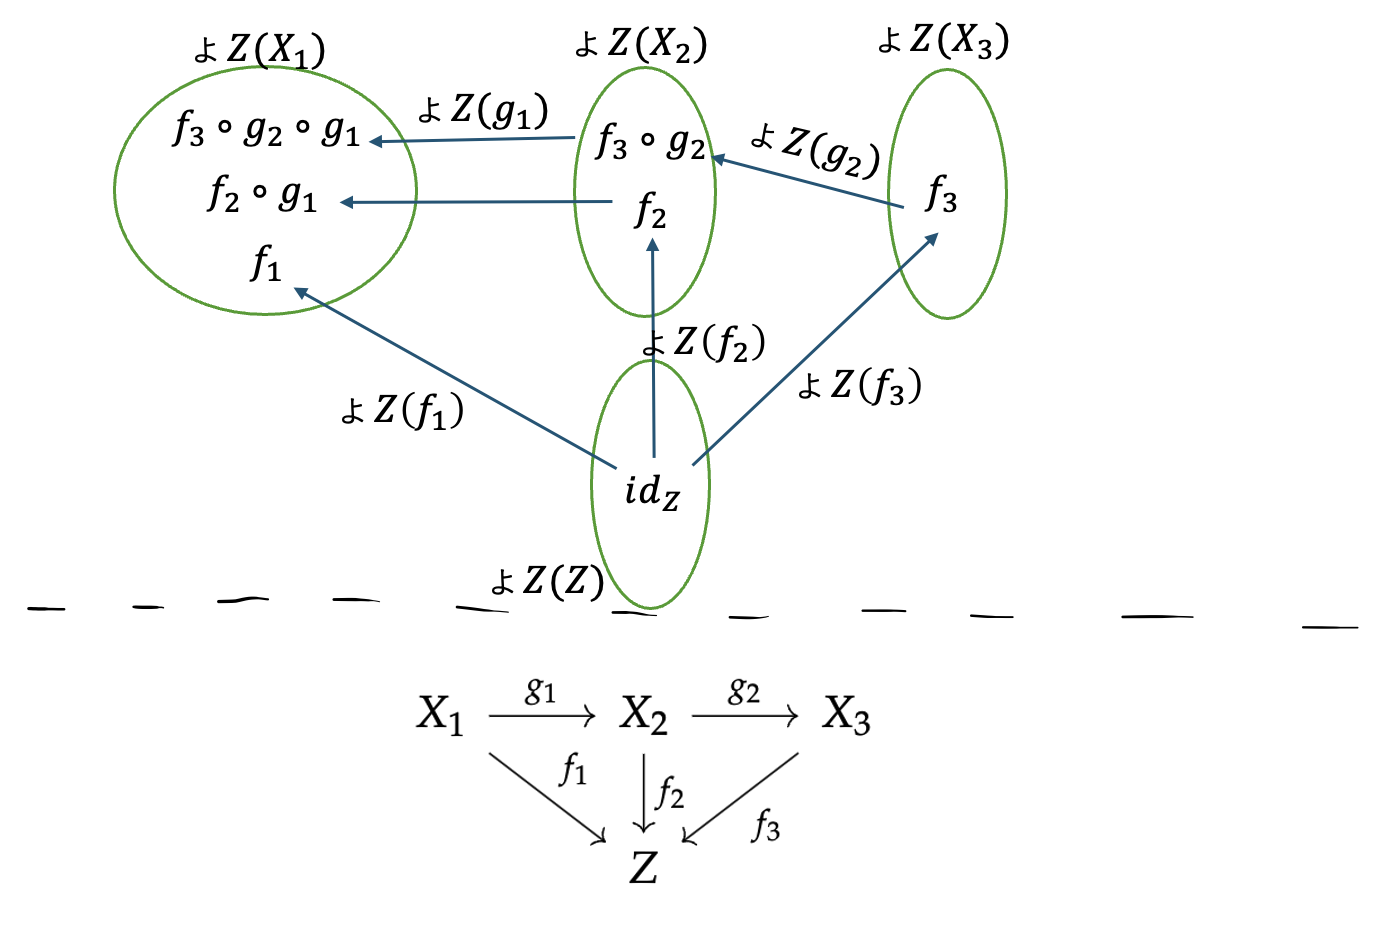
\includegraphics[width=300px]{fig/yo-1.png}
\end{center}

To build intuition, you should think of $\yo Z$ as describing ``the perspective
every other object in $\calC$ has on $Z$.'' Unpacking this more:
\begin{itemize}
  \item Let's look at the action of $\yo Z$ on $Z$ first.
  Unfolding the definition, we have:
  \begin{align*}
    (\yo Z)(Z) = \calC(Z, Z) = \{\id_Z\}
  \end{align*}
  So, somewhat vacuously, we might say: ``the perspective $Z$ has on itself 
  is the identity morphism''.
  And, for $X_1$, we have:
  \begin{align*}
    (\yo Z)(X_1) = \calC(X_1, Z) = \{f_1, f_2 \circ g_1, f_3 \circ g_2 \circ g_1 \}
  \end{align*}
  This is slightly more interesting: we would say, ``$X_1$ 
  has 3 perspectives on $Z$: (1) via the $f_1$ morphism, (2) by following 
  $f_2 \circ g_1$; (3) by following $f_3 \circ g_2 \circ g_1$''.
  \item Now let's look at the action on morphisms. These will correspond 
  to ``changes in perspective''. Let's examine the action of $\yo Z$ 
  on the morphism $f_1$:
  \begin{align*}
    (\yo Z)(f_1 : X_1 \to Z) &: \yo Z \to \yo X_1\\
    &= \id_Z \mapsto \id_z \circ f_1 = f_1
  \end{align*}
  One can understand this as: ``to move from ``$X_1$'s perspective on $Z$ 
  to $Z$'s perspective on $Z$, follow the $f_1$ morphism''. Somewhat 
  more interestingly, we can also shift perspectives between $X_1$
  and $X_2$ by precomposing with the $g_1$ morphism:
  \begin{align*}
    (\yo Z)(g_1 : X_1 \to X_2) &: (\yo Z)(X_2) \to (\yo Z)(X_1)\\
    &=
    \begin{cases}
      f_2 \mapsto f_2 \circ g_1 \\
      f_3 \circ g_2 \mapsto f_3 \circ g_2 \circ g_1
    \end{cases}
  \end{align*}
\end{itemize}

\subsection{Representables in the divisibility category}
Let's consider what representables look like in a familiar
category to get a better sense of their properties. Consider 
the following subset of the natural numbers ordered by 
divisibility:

\begin{center}
  % https://tikzcd.yichuanshen.de/#N4Igdg9gJgpgziAXAbVABwnAlgFyxMJZAJgBoAGAXVJADcBDAGwFcYkQBGYkAX1PUy58hFB1IdqdJq3YA2XvxAZseAkXKlikhizaIQ3PgJXCiZLTR0z9AZgXGhalDc3bpekAFZ7SwapEkpDZuuuwcvJIwUADm8ESgAGYAThAAtkieNDgQSGRSofoAxj7JaRlZOYgu+dYgAEYlKemImSDZSAAsNIz0dTCMAAp+pvqMMAk4IJbu7PSNZYh57YhiNR5Q883Vy6tWHmxGIKXNq8saa+wJETxAA
\begin{tikzcd}
  &                   & 12                                                &   \\
  & 6 \arrow[ru, "f"] &                                                   &   \\
2 \arrow[ru, "d"] &                   & 3 \arrow[lu, "e"]                                 & 5 \\
  &                   & 1 \arrow[llu, "c"] \arrow[u, "b"] \arrow[ru, "a"] &  
\end{tikzcd}
\end{center}

Let's consider the representables of each element in this category.
First let's inspect $\yo 12$. We can compute its action on objects:
\begin{align*}
  (\yo 12)(12) = \{\id_{12}\} \quad&
  (\yo 12)(6) = \{f\} \quad&
  (\yo 12)(3) = \{f \circ e\} \\
  (\yo 12)(2) = \{f \circ d\} \quad&
  (\yo 12)(1) = \{f \circ d \circ c\} \quad &
  (\yo 12)(5) = \{\}
\end{align*}

Note that in this category there is at most 1 morphism between any 2 objects
(i.e., we have that the morphisms $f \circ d \circ c = f \circ e \circ b$, 
so we only include 1 of them in $(\yo 12)(1)$).  So, each representable $\yo X$ is either a singleton (meaning, $X \preceq
12$), or it is an empty set (meaning $X \not\preceq 12$). The action of $\yo 12$
on morphisms is not complicated, let's see what it is by unfolding definitions:
\begin{align*}
  (\yo 12)(c) &: (\yo 12)(2) \to (\yo 12) (1) \\
  &= (f \circ d) \mapsto (f \circ d) \circ c
\end{align*}

In this case we see that to shift perspective from $1$ to $2$, we should 
precompose by the $c$ morphism.
From this, we can observe that there is single morphism $\yo Y \to \yo X$ 
if and only if there is a morphism $X \to Y$ in $\calC$.

Now, let's closely examine the structure of a representable $\yo 12$ and try 
to gain a more global picture of what data it contains. We can summarize 
$\yo 12$ by the following balloon, where we've replaced each object 
by its balloon:

\begin{center}
  % https://tikzcd.yichuanshen.de/#N4Igdg9gJgpgziAXAbVABwnAlgFyxMJZAJgBoAGAXVJADcBDAGwFcYkQAdD4LuHegE5cAviGGl0mXPkIoAjKTnU6TVuy48OfQSLESQGbHgJFypYsoYs2iTt178hHUeMlGZRMhZpW1tjQ46znpu0iYoZADMlqo2dpraTi76hmGyyAAs5jHW6vbBwsowUADm8ESgAGYCEAC2SGYgOBBIcq4g1XWtNM1IxO2d9YgKTS2IkQM1Q2SjSBmTXeM9Y-P6g0gArMtzhcJAA
\begin{tikzcd}
  &                                 & \{\star\} \arrow[ld] &  &                  \\
  & \{\star\} \arrow[ld] \arrow[rd] &                      &  &                  \\
\{\star\} \arrow[rrd] &                                 & \{\star\} \arrow[d]  &  & \{\} \arrow[lld] \\
  &                                 & \{\star\}            &  &                 
\end{tikzcd}
\end{center}

We see that the collection of objects with a $\star$ in them are exactly those objects 
that are at or below 12 in the order. This collection of objects has a name in 
order theory: it is called the \textbf{principal ideal} of 12. Formally:

\begin{definition}[Principal ideal]
  Let $(X, \le)$ be a preorder. Then, the \textbf{principal ideal} 
  of an element $a \in X$, written $\downarrow a$, 
  is the smallest collection of all elements less than or equal to $a$ 
  in $X$, i.e. 
  $\downarrow a = \{x \in X \mid x \le a\}$.
\end{definition}

So, we can summarize:
the representable $\yo 12$ is the principal ideal $\downarrow 12$, i.e.,
it contains exactly as much information as is contained in the principal ideal of 12. In general,
for any category formed by a preorder, it is the case that the representable of an 
element is a principal ideal in the preorder.
This order-theoretic viewpoint sheds some light on the intuition that the representable of an 
element is ``all the ways of viewing the element in the category''. One can imagine 
``peering up'' at an element $X$ from all the other objects: $\yo X$ is then all the vantage points below $X$ from 
which it can be seen.

\section{Representables in STLC}
So far we've been studying representables in thin categories, where there is a 
very pleasant order-theoretic understanding what they mean in terms of principal ideals.
Let's see an example of representables in a category with more than 1 morphism 
between objects.
Recall the syntax of \textsc{stlc}:
\begin{gather}
  \begin{aligned}
   A,B &::= \plkw{Unit}
     \mid A \pltimes B
     \mid A \plto B
  \\
  M,N &::= \plunit{}
      \mid \plpair{M}{N}
      \mid \plfst{M}
      \mid \plsnd{M}
      \mid \pllam{x}{M}
      \mid \plapp{M}{N}
      \mid x
  \end{aligned}
  \tag{\textsc{stlc}}
\end{gather}

Recall the category of simply-typed lambda calculus terms quotiented by 
equations:
\begin{definition}[The category STLC]
  The category of simply-typed lambda calculus terms (\textsc{stlc}) 
  is the category where:
  \begin{itemize}
    \item Objects are types $A$;
    \item Morphisms $A \to B$ are equivalence classes of terms $[x : A \vdash e : B]$ 
    where equality is given by the equational theory of the $\beta$ and $\eta$ laws;
    \item Composition is given by substitution:
    \begin{align*}
      [b : B \vdash N : C] \circ [a : A \vdash M : B] = [a : A \vdash N[M/b] : C]
    \end{align*}
    \item The identity morphism is the class of terms $[a : A \vdash a : A]$.
  \end{itemize}
\end{definition}

Let's see the representables in this category. 
For example, what do the representables $\yo (\plUnit \times \plUnit)$ look like?
Considering a concrete example:
\begin{align*}
  \yo (\plUnit \times \plUnit)(\plUnit) 
  &= \{\text{the ways of viewing terms of type $\plUnit \times \plUnit$ from terms of type $\plUnit$}\} \\ 
  &= \{[a : \plUnit \vdash M : \plUnit \times \plUnit] \mid M \text{ an stlc term}\}\\ 
  &= [a : \plUnit \vdash \plpair{a}{a} : \plUnit \times \plUnit]
\end{align*}

In the case above, there is only 1 element of the set $\yo (\plUnit \times \plUnit)(\plUnit)$: 
this is a quirk of our choice of types.
Intuitively, the representables $(\yo B)(A)$ for two types $A$ and $B$ 
is the collection of all equivalence classes of terms $M$ of type $A \to B$.
Then, naturally, the action on morphisms $(\yo X)(f : A \to B) : \yo B \to \yo A$ 
ought to be the ways of shifting viewpoints from $B$ to $A$,
i.e.:

\begin{align*}
  (\yo X)([a : A \vdash M : B]) &: (\yo X)(B) \to (\yo X)(A) \\
  &= [b : B \vdash N : X] \mapsto [b : B \vdash N : X] \circ [a : A \vdash O : B]  \\
  &= [b : B \vdash N : X] \mapsto [a : A \vdash N[O/b] : X]
\end{align*}

Carefully check all the types in the above equations.

\section{Representability}

There can be many $\calC$-indexed sets for a category, but the representables
are very special due to their relationship with the indexing category.
As usual in category theory, we are concerned not with particular objects 
but rather with equivalence classes of objects up to isomorphism,
a notion we make formal here:

\begin{definition}[Isomorphism of $\calC$-indexed sets]
  Two \(\calC\)-indexed sets \(P,Q\)
  are \emph{isomorphic}
if there are \(\calC\)-indexed functions \(\alpha : P \Rightarrow Q\)
and \(\beta : Q \Rightarrow P\)
such that \(\alpha\circ\beta=\idt_Q\) and \(\beta\circ\alpha=\idt_P\).
\end{definition}

With this definition in hand we can make precise the set of $\calC$-indexed 
sets that are tied to the indexing category:

\begin{definition}[Representability]
  \sloppy
  A \(\calC\)-indexed set \(P\) is \emph{representable}
  if there is an isomorphism \(\alpha : P \cong \yo X : \beta\)
  for some object \(X\) of \(\calC\).
\end{definition}

\begin{proposition}
  The \(\FinSet\)-indexed set \(\yo X \times \yo Y\)
  is representable.
\end{proposition}
\begin{proof}
  for any finite set \(A\), there is an isomorphism of sets
  \[
  \alpha_A : \FinSet(A,X \times Y) \cong \FinSet(A,X) \times \FinSet(A,Y).
  \]
  Concretely, \(\alpha_A\) is the function that sends
  a \(f \in \FinSet(A,X\times Y)\) to \((\pi_1 \circ f ,\pi_2,\circ f): \FinSet(A,X) \times \FinSet(A,Y) \).
  Its inverse is defined by \(\beta_A(f,g) = \angled{f,g}\).
  Both \(\alpha\) and \(\beta\) can be checked satisfy the naturality condition.
  Thus \(X\times Y\) represents \(\yo X \times \yo Y\).
\end{proof}

Representability is the bridge between
the internal view and the external view of a category: it lets us reflect 
properties presheaf category on $\calC$ back into $\calC$ itself. Concretely,
in the next chapter, we will use the Yoneda lemma in full to show:

\begin{theorem}
  Let $P,A,B$ be objects in a category $\calC$.  Then, $P$ is a product of $A$
  and $B$ if and only if it represents the product in the presheaf category $\yo A \times \yo B$.
\end{theorem}

We will not prove this theorem here -- it is a direct consequence of the 
Yoneda lemma, which we are now ready to appreciate -- but
one can understand this theorem as: an object $P$ is a product of $A$ 
and $B$ internally if and only if if behaves like a product externally.

% \section{The category of elements}

%% \section{$\calC$-indexed sets}

%% Let's begin by studying the category $\mathbb{N}^\infty$, the category
%% constructed from the preorder formed by the natural numbers extended by
%% infinity:

%% \begin{center}
%% \begin{tikzpicture}[
%% ]
%% % Objects (circles)
%% \node[minimum size=0.6cm] (o1) at (0,-1) {0};
%% \node[minimum size=0.6cm] (o2) at (1.5,-1) {1};
%% \node[minimum size=0.6cm] (o3) at (3,-1) {2};
%% \node (dots) at (4.2,-1) {$\cdots$};

%% % Arrows between objects
%% \draw[->] (o1) -- node[above] {$f$} (o2);
%% \draw[->] (o2) -- node[above] {$g$} (o3);
%% \draw[->] (o3) -- (dots);

%% \draw[->] (o1) edge[loop above] node[above] {$\id_0$} (o1);
%% \draw[->] (o2) edge[loop above] node[above] {$\id_1$} (o2);
%% \draw[->] (o3) edge[loop above] node[above] {$\id_2$} (o3);
%% \end{tikzpicture}
%% \end{center}

%% Given a category $\calC$, a $\calC$-indexed set associates each object of
%% a category with a set.
%% Let's consider a concrete $\calC$-indexed set called $F$.
%% We can draw $F$ as a ``balloon picture'' like this:

%% \begin{center}
%%   \includegraphics[width=175px]{fig/balloon-1.png}
%% \end{center}

%% Above each object is drawn a (in this case, finite) set.
%% $F_1$ is the set $\{a, b, c\}$, and $F_2$ is is the set
%% $\{d, e\}$.
%% In addition to associating each object with a set,
%% a $\calC$-indexed set also associates each morphism $X \mor{f} Y$
%% with a function $F_Y \to F_X$, which we can draw on the balloon
%% picture like so:

%% \begin{center}
%% \includegraphics[width=175px]{fig/balloon-2.png}
%% \end{center}

%% Intuitively, we can see that $F$ is describing a relation between two
%% categories: our category of interest $\calC$, and an ``external''
%% category of sets and functions. This relation is called a \textbf{functor}.
%% Functors have actions on objects

% \begin{tikzpicture}[
%   node distance=1.5cm,
%   morphism/.style={-Stealth, thick}
% ]

% % Top row of labels
% \node (v) at (0,2) {$v$};
% \node (c) at (3,2) {$c$};

% % Middle row
% \node (y) at (-1.5,1) {$y$};
% \node (w) at (0,1) {$w$};
% \node (a) at (3,1) {$a$};

% % Bottom row (just above the objects)
% \node (x) at (-1.5,0) {$x$};
% \node (h) at (0,0) {$h$};
% \node (b) at (3,0) {$b$};

% % Objects (circles)
% \node[circle, draw, minimum size=0.6cm] (o1) at (0,-1) {0};
% \node[circle, draw, minimum size=0.6cm] (o2) at (1.5,-1) {1};
% \node[circle, draw, minimum size=0.6cm] (o3) at (3,-1) {2};
% \node (dots) at (4.2,-1) {$\cdots$};

% % Arrows between objects
% \draw[morphism] (o1) -- (o2);
% \draw[morphism] (o2) -- (o3);
% \draw[morphism] (o3) -- (dots);

% \end{tikzpicture}




% \begin{center}
%  \begin{tikzpicture}[]

% % Objects
% \node (A) at (0,0) {$A$};
% \node (B) at (3,0) {$B$};
% \node (C) at (1.5,2.5) {$C$};

% % Identity morphisms (loops)
% \draw[->] (A) edge[loop left] node[left] {$\text{id}_A$} (A);
% \draw[->] (B) edge[loop right] node[right] {$\text{id}_B$} (B);
% \draw[->] (C) edge[loop above] node[above] {$\text{id}_C$} (C);

% % Morphisms between objects
% \draw[->] (A) -- node[below] {$f$} (B);
% \draw[->] (A) -- node[left] {$g$} (C);
% \draw[->] (C) -- node[right] {$h$} (B);
% \node[draw, fit=(A)(B)(C), inner sep=1cm, rectangle] {};
% \end{tikzpicture}
% \end{center}


%% Throughout this section we will work with an arbitrary category \(\calC\).

%% \begin{definition}[$\calC$-indexed set]
%%   A $\calC$-indexed set is a functor $F : \calC^\text{op} \Rightarrow \Set$.
%% \end{definition}

%% \begin{example}
%%   Recall that \(\mathsf{STLC}\) is a category
%%   whose objects are types and whose morphisms \(A \to B\)
%%   are terms \(x : A \vdash M : B\) quotiented by \(\beta\eta\)-equivalence.
%%   For each type \(A\),
%%   the following defines a \(\mathsf{STLC}\)-indexed set \(\mathsf{Tm}(A)\):
%%   \begin{align}
%%   \mathsf{Tm}(B)(A) &= \text{the set of morphisms \(A\to B\)} \\
%%   \mathsf{Tm}(B)(N : A'\to A)
%%   &= (x\ofty A \vdash M : B) \mapsto (x'\ofty A' \vdash M[N/x] : B)
%%   \end{align}
%% \end{example}
%% This example is a special case of a canonical kind of \(\calC\)-indexed set.
%% \begin{definition}
%%   The \emph{representable \(\calC\)-indexed set at \(X\)}
%%   is written \(\yo X\) and defined by
%%   \begin{align}
%%     (\yo X)(A) &= \text{the set of morphisms \(A \to X\)} \\
%%     (\yo X)(A)(s : A' \to A) &= (f : A \to X) \mapsto (f \circ s : A' \to X)
%%   \end{align}
%% \end{definition}

%% \begin{definition}
%%   \sloppy
%%   Let \(P\) and \(Q\) be \(\calC\)-indexed sets.
%%   A \emph{\(\calC\)-indexed function}
%%   from \(P\) to \(Q\),
%%   written \(\alpha : P \Rightarrow Q\),
%%   is a family of functions \(\alpha_X : PX \to QX\)
%%   that ``respects substitution''
%%   in the sense that \(\alpha_{X'}(x\cdot_P p) = \alpha_X(x)\cdot_p p\).
%% \end{definition}

%% \begin{itemize}
%% \item \(\calC\)-indexed functions can be composed:
%%   the composition of \(\alpha : Q \Rightarrow R\)
%%   and \(\beta: P \Rightarrow Q\),
%%   written \(\alpha\circ\beta : P \Rightarrow R\),
%%   is defined by \((\alpha\circ\beta)_X = \alpha_X \circ \beta_X\).
%% \item For each \(\calC\)-indexed set \(P\),
%%   there is a \(\calC\)-indexed function \(\idt_P : P \Rightarrow P\)
%%   defined by \(\idt_{P,X} = \left(PX \xrightarrow{\idt_{PX}} PX\right)\).
%% \end{itemize}
%% By now you may have noticed that \(\calC\)-indexed sets and functions
%% look like they ought to form a category. More on this later.

%% \begin{definition}
%%   Two \(\calC\)-indexed sets \(P,Q\)
%%   are \emph{isomorphic}
%% if there are \(\calC\)-indexed functions \(\alpha : P \Rightarrow Q\)
%% and \(\beta : Q \Rightarrow P\)
%% such that \(\alpha\circ\beta=\idt_Q\) and \(\beta\circ\alpha=\idt_P\).
%% \end{definition}

%% \begin{definition}
%%   A \(\calC\)-indexed set \(P\) is \emph{representable}
%%   if there is an isomorphism \(\alpha : P \cong \yo X : \beta\)
%%   for some object \(X\) of \(\calC\).
%% \end{definition}


\chapter{Yoneda IV: universal constructions, elements, and properties}

Now we are ready to appreciate the Yoneda lemma:

\begin{theorem}[Baby Yoneda]
  Let $\calC$ be a category, $X$ be an object in $\calC$, and $P$ 
  be a $\calC$-indexed set. Then, there is a bijective correspondence:\footnote{This 
  is called the ``baby Yoneda lemma'' because the full Yoneda lemma further stipulates 
  that this isomorphism satisfies additional naturality conditions. The baby Yoneda 
  lemma is still quite strong, however, and is much easier to prove.}
  \begin{align*}
    \{\text{$\calC$-indexed functions }\yo X \Rightarrow P\} \cong P(X)
  \end{align*}
  \label{thm:baby-yo}
\end{theorem}

On first glance this theorem is profoundly mysterious because it stipulates 
that there is a very strong relationship between two very different-seeming 
things. Let's unpack this slowly to really understand what is going on 
by instantiating the Yoneda lemma to a specific category and 
$\calC$-indexed set.
Let's consider a finite category with 3 objects:

\begin{equation}
  % https://tikzcd.yichuanshen.de/#N4Igdg9gJgpgziAXAbVABwnAlgFyxMJZABgBpiBdUkANwEMAbAVxiRAA0QBfU9TXfIRQBGclVqMWbAJrdeIDNjwEiAJjHV6zVohAAtbuJhQA5vCKgAZgCcIAWyRkQOCEmE8rth4lHPXiVS4KLiA
\begin{tikzcd}
  X \arrow[r, "f"] & Y \arrow[r, "g"] & Z
  \end{tikzcd}
\end{equation}

Now, let's define a simple $\calC$-indexed set $P$:
\begin{align*}
  P(X) = \{a, b\} \quad 
  P(Y) = \{c, d\} \quad
  P(Z) = \{e, h\} \\
  P(f) = \begin{cases}
    c \mapsto a \\
    d \mapsto b
  \end{cases}
  \quad 
  P(g) = \begin{cases}
    e \mapsto c \\
    h \mapsto d
  \end{cases}
\end{align*}

Continuing to unpack the data, we can define $\yo Z$, which is 
also a $\calC$-indexed set:

\begin{align*}
  (\yo Z)(Z) = \{\id_Z\} \quad
  (\yo Z)(Y) = \{g\} \quad
  (\yo Z)(X) = \{g \circ f\}
  \\
  (\yo Z)(f) = g \mapsto f \circ g \quad
  (\yo Z)(g) = \id_Z \mapsto f
\end{align*}

Next, let's enumerate the natural transformations $\yo X \Rightarrow P$
If the Yoneda lemma is true, we don't have too much work to do: 
we know there should be \emph{only two of them}, since $P(X)$ 
has only two elements in it. Let's enumerate them on a balloon diagram:

\begin{fullwidth}
  \begin{center}
    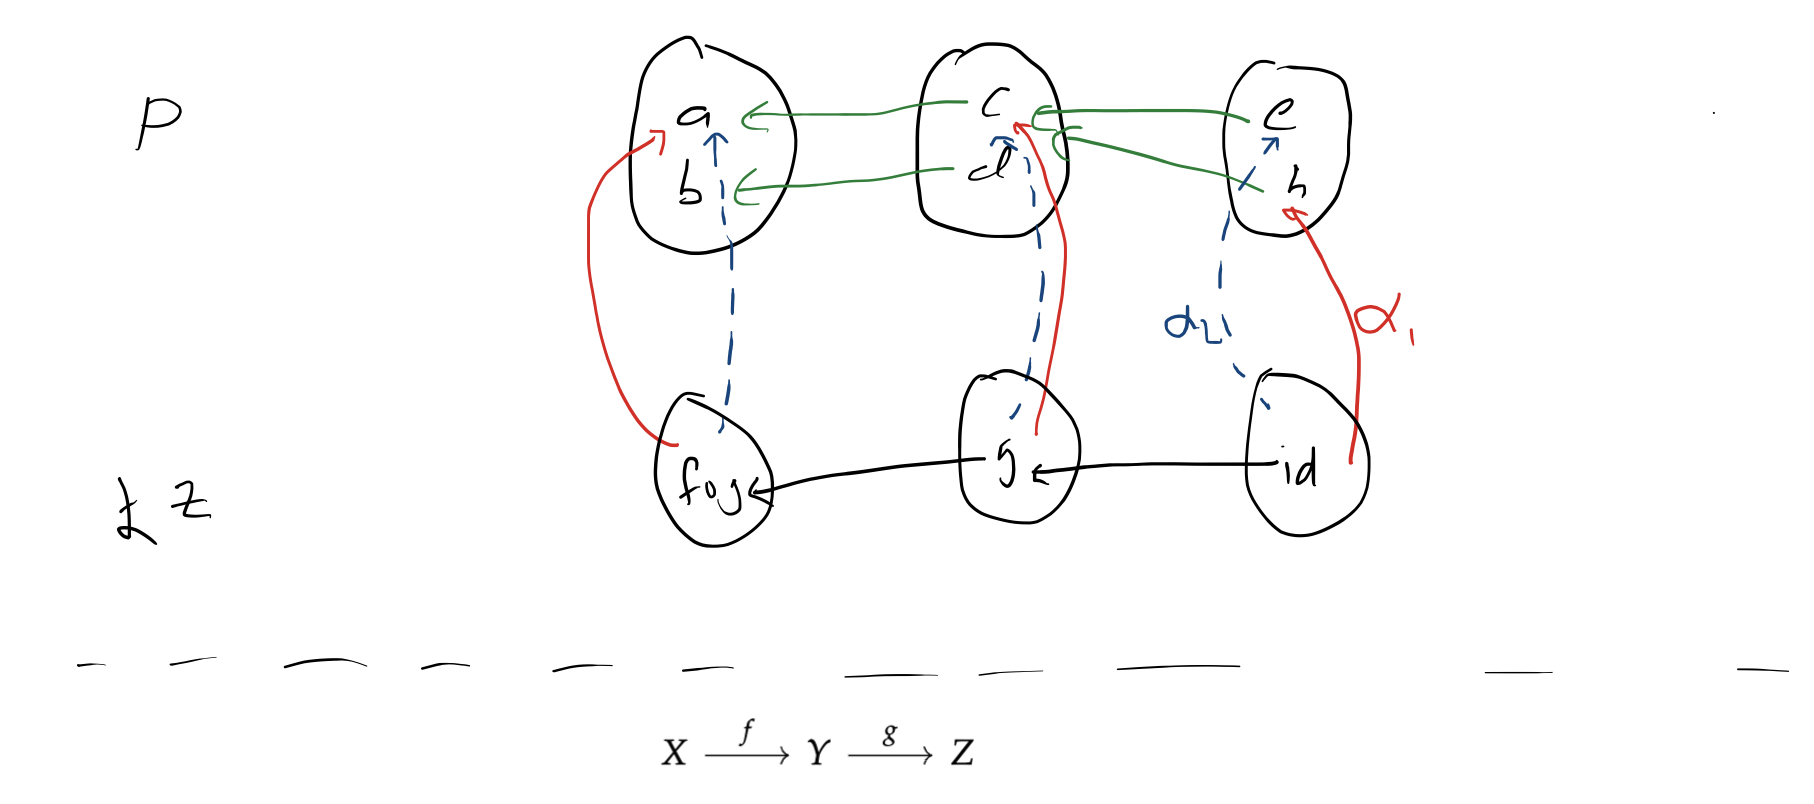
\includegraphics[width=400px]{fig/yo-2.png}
  \end{center}
\end{fullwidth}

Here we've drawn the two possible natural transformations $\alpha_1$ and
$\alpha_2$ in solid red and dashed blue respectively.  Now, let's understand why
the Yoneda lemma holds by tracing the possible paths through this balloon
diagram with your fingers.  Recall the two finger rule: a $\calC$-indexed
function $\yo Z \Rightarrow P$ satisfies the naturality condition if, starting
at any element in any balloon $\yo X$, your two fingers move in synchrony along
all possible paths.
So, let's start with $\yo Z = \{\id_Z\}$. Let's play the two finger game together
to design the two possible natural transformations:
\begin{itemize}
  \item Your left finger moves to $g$. Where can your right finger go? 
  It can go either to $e$ or $h$. So, choose $h$ and so we are designing $\alpha_1$. \emph{The rest of the 
  moves are forced}: your right finger must now move to $c$,
  then to $a$. Your left finger is also forced: it must move to $g$ 
  then to $f \circ g$. Now, all other decisions are forced, and we 
  can fill in $\alpha_1$ so that all moves are in harmony.
  \item Next, we can choose moving our right finger to $e$, and so 
  we are designing $\alpha_2$. \emph{Again, all moves are forced}: 
  the right finger follows the functions in $P$, and the left finger 
  follows the functions in $\yo Z$. Then, we are forced to choose 
  each $\alpha$ to exactly line up exactly with how these fingers move: 
  there is only one choice for $\alpha$ at each step.
\end{itemize}

Notice what is happening: because, in this example, 
there is a single element in $(\yo Z)(Z)$, then there must be 
\emph{exactly 1} natural transformation for each possible 
element in $P(Z)$. Naturality is a very strong restraint 
to place on $\alpha$!

So, it is now hopefully quite clear that, if $\id_Z$ is the only element of $\yo
Z$, the baby Yoneda lemma is true, since the entire action of a natural
transformation is determined by its action on the identity morphism of $Z$. But,
what if there is more than one morphism in $(\yo Z)(Z)$?

The crux is that the choice of \emph{$(\yo Z)(\id_Z)$} fully determines the
action of $\yo Z$ on all the other morphisms $Z \to Z$. Let's see this visually. 
Suppose we have as our indexing category the monoid corresponding to the 
natural numbers mod 3 under addition. This category has a single object $\star$ and 
3 morphisms: the identity morphism $0$, $1, 2$, where $1 \circ 1 = 2, 1 \circ 2 = \id, 2 \circ 2 = 1, 2 \circ 1 = \id$.
Let's visualize some of this data:

\begin{center}
  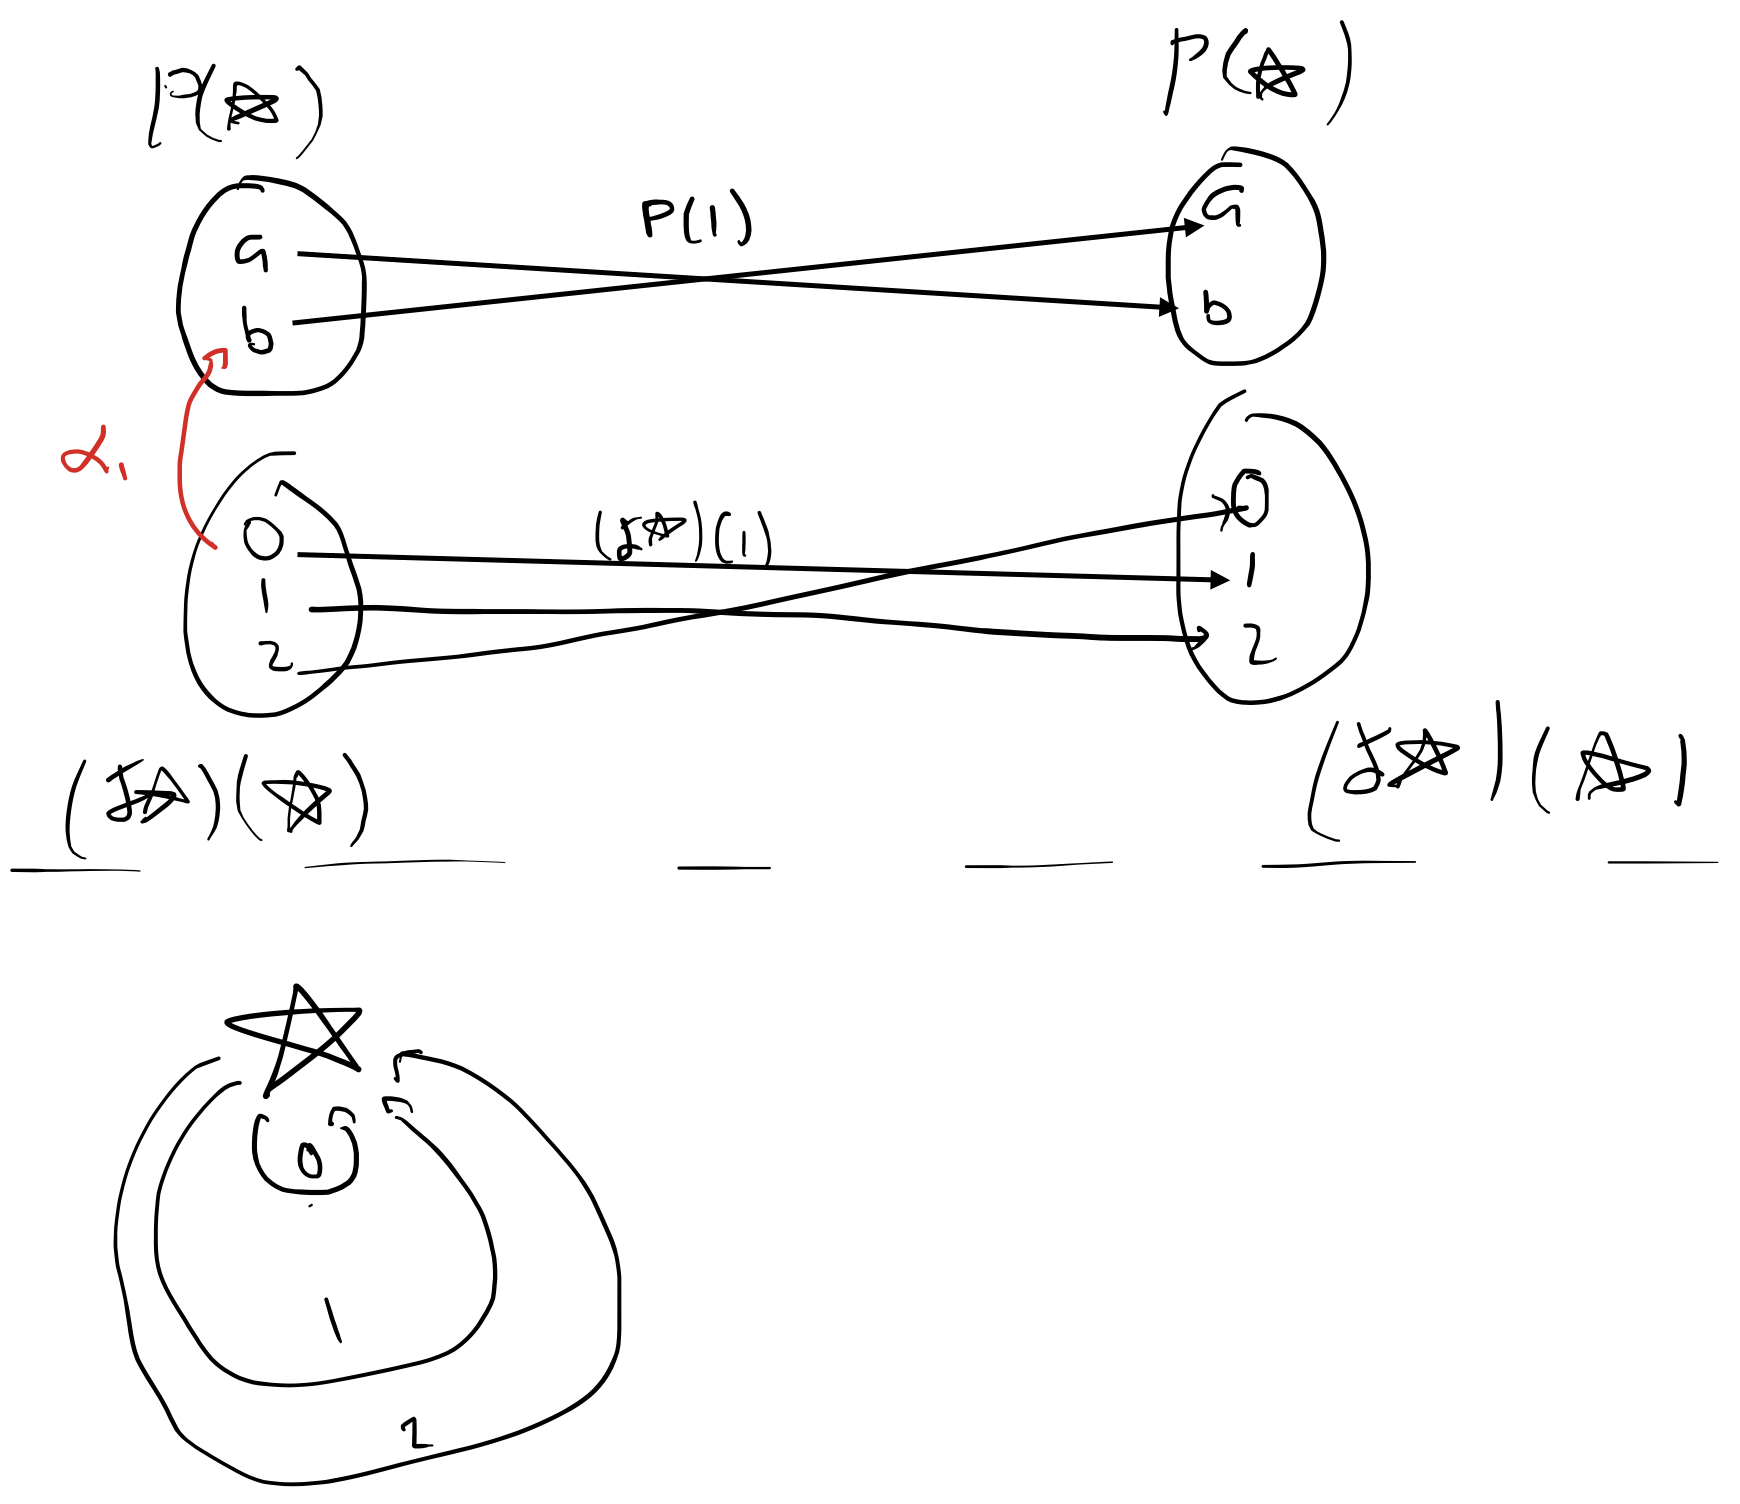
\includegraphics[width=250px]{fig/yo-3.png}
\end{center}

Here we've drawn an arbitrary $\calC$-indexed set $P$
with its action on the $1$ morphism, and we've chosen arbitrarily that
the $\calC$-indexed function
$\alpha_1$ maps $0$ to $b$. 
Note that we've drawn the balloon twice for the same object; this is for visualization 
purposes only.
Now, the key: \emph{does this choice of $\alpha$ 
fully determine how $\alpha$ behaves on all other elements of $(\yo \star)(\star)$}?
Indeed it does! Observe: by naturality, we have that $\alpha_1(1) = a$, which 
we can see by composing $P(1)\circ\alpha_1$. This gives us one more piece of data 
about $\alpha_1$. Now, what about $\alpha_1(2)$? We can get this piece of data 
by inspecting $P(2)$ and $(\yo \star)(2)$:

\begin{center}
  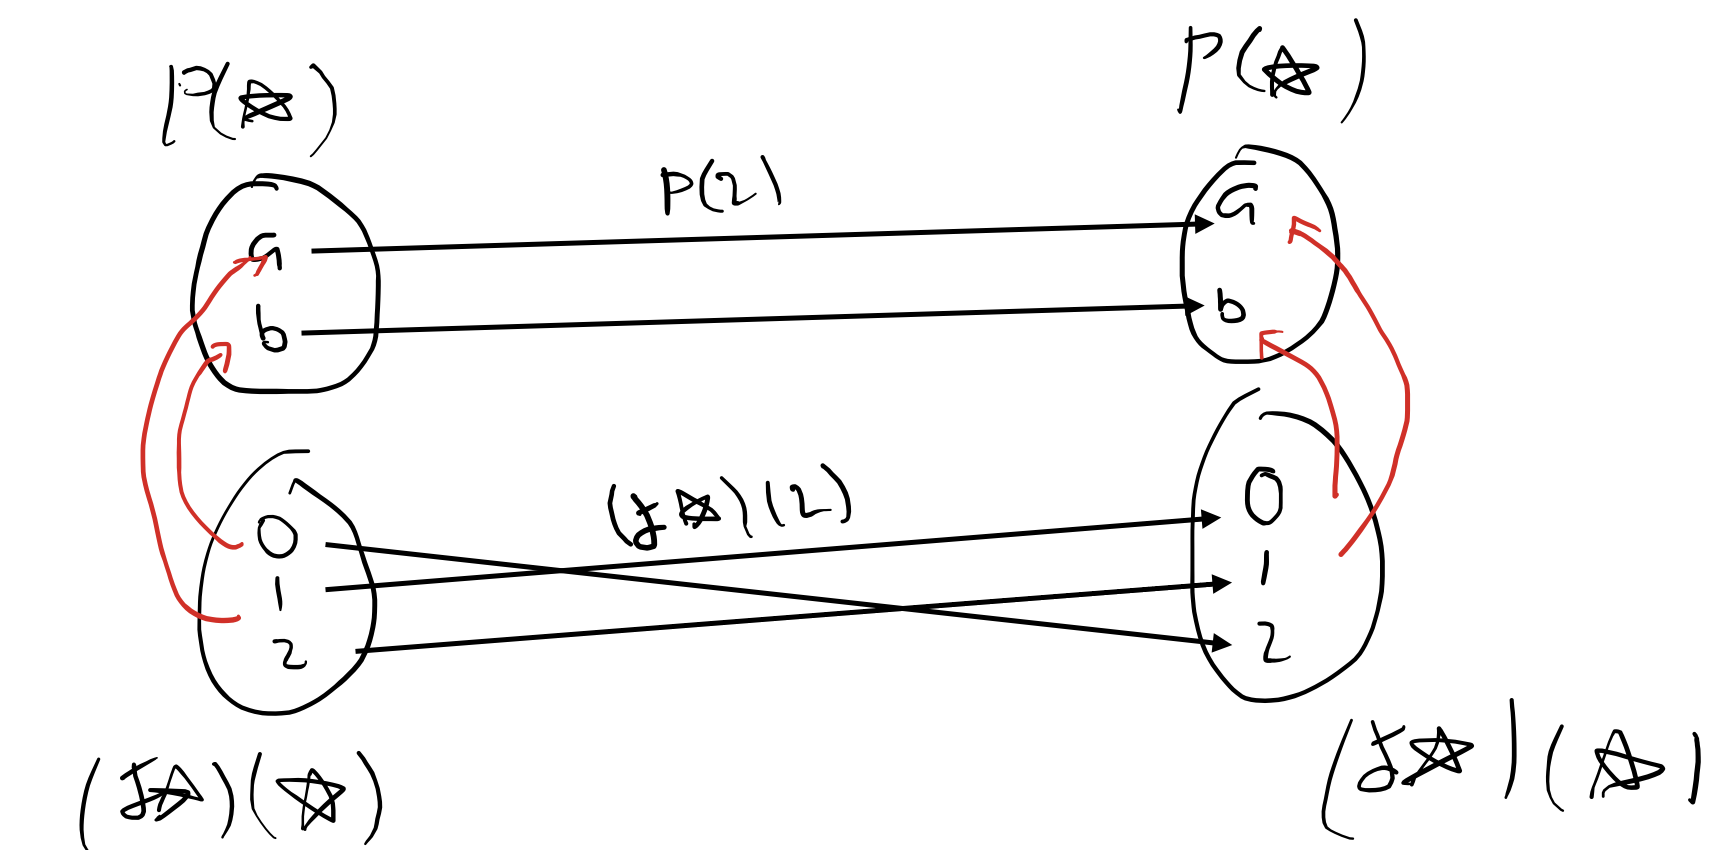
\includegraphics[width=250px]{fig/yo-4.png}
\end{center}

And now here we learn the final component of $\alpha$: we conclude that $\alpha(2) = b$.

\section{Proving the baby Yoneda lemma}
\marginnote{Thanks to Bex Golinov for the scribe notes for the next two subsections. \todo{} these can be tidied 
up a bit.}
Now we are ready to prove \cref{thm:baby-yo}. Let $\calC$ be a 
category, $P$ be a $\calC$-indexed set, and $X$ be an object 
in $\calC$. Then, we need to construct a bijection:

\begin{center}
  % https://tikzcd.yichuanshen.de/#N4Igdg9gJgpgziAXAbVABwnAlgFyxMJZABgBpiBdUkANwEMAbAVxiRAB13hOBfEH0uky58hFAEZyVWoxZsACgAoAGgEp+0mFADm8IqABmAJwgBbJGRA4ISSSABGMMFCQBmS-WatEIbf0Egxma21NYW1I7ObpYMdI4M8sJ4BGwMMAY4INSecj4GTGAAxho8QA
\begin{tikzcd}
  \{\calC\text{-indexed functions }\yo X \Rightarrow P\} \arrow[r, "g", bend left] & P(X) \arrow[l, "func", bend left]
  \end{tikzcd}
\end{center}

\newcommand{\fun}{func}
\newcommand{\cat}{\mathcal{C}}
What does this bijective correspondence statement actually mean? We have some
$\fun$ that, given a $p\in PX,$ can construct a natural transformation $\alpha:
\yo X \Rightarrow P$, and some $g$ that can extract $p$ from a given natural
transformation.
\begin{enumerate}
    \item Constructing natural transformation from $p\in PX$
    \begin{itemize}
        \item Given a $p\in PX$, we defined
        $\fun(p)$ via a family of functions $\fun(p)_A,$ where $\fun(p)$ is a
        natural transformation. We can think of the $\fun(p)_A$ as the
        components of $\fun(p),$ where for each object $A$ in $\cat,$ the
        component $\fun(p)_A$ maps from $(\yo X )(A)$ to $P(A)$. 
    \begin{align*}
        \fun(p)_A : &(\yo X)(A) \to PA\\
        &f \mapsto (Pf)(p)
    \end{align*}
    where $f:A \to \yo X$. The element $p$ by definition has type $PX,$ and $P$ is contravariant so $Pf$ maps $PX$ to $PA,$ giving us the desired codomain.
    \item Naturality of $\fun(p)$. Let $g:B\to A$. I don't really want to justify this but here is the square
    \[
\begin{tikzcd}[column sep=large, row sep=large]
(\yo X)(A) \arrow[r, "\fun(p)_A"] \arrow[d, "(\yo X)(g)"'] & P(A) \arrow[d, "P(g)"] \\
(\yo X)(B) \arrow[r, "\fun(p)_B"'] & P(B)
\end{tikzcd}
\]
    \end{itemize}
    \item Getting $p$ from natural transformation
    \begin{itemize}
    \item How did we extract $p\in PX$ from some given natural transformation $\alpha$? We know $\alpha_X$ maps $(\yo X)(X) \to PX$, so applying $\alpha_X$ to $id_X$ gives us an element of $PX,$ we can set $p:=\alpha_X(id_X)$. 
    \item Now we need to show $\alpha_A = \fun(p)_A$. Since $\alpha_A$ acts on the elements of $(\yo X)(A)$, it suffices to show $\alpha_A(f) = \fun(p)_A = (Pf)(p)$ for every $f\in\cat(A,X)$.
    \item We have $(Pf)(p) = (Pf)(\alpha_X(id_X))$. We will use the naturality of $\alpha$. Specifically, $Pf \circ \alpha_X = \alpha_A \circ (\yo X)(f)$.
      \[
\begin{tikzcd}[column sep=large, row sep=large]
(\yo X)(X) \arrow[r, "\alpha_X"] \arrow[d, "(\yo X)(f)"'] & P(A) \arrow[d, "P(f)"] \\
(\yo X)(A) \arrow[r, "\alpha_A"'] & P(B)
\end{tikzcd}
\]
    \begin{align*}
        (Pf)(\alpha_X (id_X)) = (Pf \circ \alpha_A)(id_X) &= (\alpha_A \circ (\yo X)(f))(id_X)\\
        &= \alpha_A((\yo X)(f)(id_X)) = \alpha_A(id_x \circ f).\\
        &= \alpha_A(f)
    \end{align*}
    So $(Pf)(p) = \alpha_A(f)$, and we are done!
\end{itemize}
\end{enumerate}

\begin{remark}
    Defining some natural transformation $\alpha := f(p)$ by defining how $f(p)$ acts on each object $A$ is like a "pointwise" definition of $\alpha$. 
\end{remark}

\section{The category of elements}
\begin{definition}[Category of elements]
  Let $P$ be a $\calC$-indexed set.
    The \textit{category of elements} of $P$, written $\int_C P$, is a 
    category where:
    \begin{enumerate}
        \item objects : pairs $(X,p\in PX)$
        \item morphisms : from $(X,p\in PX)$ to $(Y,q\in PY)$ are morphisms
        $f:X\to Y$ of $\cat$ such that $(Pf)(q) = p$. Alternatively, $q \cdot_P
        f = p$. A morphism of this category of elements is a morphism from the
        original category with the \textit{additional} structure of preserving
        the points of $PX$.
    \end{enumerate}
    Definitions of composition and identity follow immediately from the
    definitions in $\cat,$ with the additional restriction of point
    preservation. It is relatively simple to show the desired categorical
    properties hold.
\end{definition}
\begin{proposition}
    Suppose $\cat$-indexed set $P$ is representable by $X$. There exists a $u\in
    PX$ called the \textit{P-universal element} which satisfies the following
    universal property : for any object $\Gamma$ of $\cat$ and any $g\in
    P\Gamma,$ there exists a unique $\hat{g}:\Gamma\to X$ such that $g = u
    \cdot_P \hat{g}$. Alternatively, $g = (P\hat{g})(u)$.
    \label{prop:univ-elem}
\end{proposition}
\begin{proposition}
    A $\cat$-indexed set $P$ is representable if $P\cong\yo X$ for some object
    $X$ of $\cat$. Suppose $P$ is representable. Then there exists a
    \textit{universal element} $u\in PX$ and $u$ is a terminal object in the
    \textit{category of elements} of $P$.
    \label{prop:univ-terminal}
\end{proposition}

We have from \cref{prop:univ-terminal} the definition of the universal property that we
want these mysterious universal elements to satisfy. We can think about this
definition as stating that we can ``factor'' any $g\in P\Gamma$ (for any $\Gamma$)
into $u$ and a unique $\hat{g}$.


What does it mean for $u \in P(X)$ to be terminal in the category of elements of
$P$? That any object has a unique morphism mapping to $(X,u)$. Explicitly, for
any $(A, p\in PA),$ there is a unique map $f:A \to X$ such that $(Pf)(u)=p$ (or
$p = u \cdot_P f)$. This looks pretty similar to the universal property given in
\cref{prop:univ-terminal} -- we can ``factor'' any $p\in PA$ into $f$ and $u$.


How do we get \cref{prop:univ-terminal} from the Yoneda Lemma? These are the key ideas:
\begin{itemize}
    \item $X$ representing $P$ means we have an isomorphism between $\yo X$ and $P$. This isomorphism is a $\cat-$indexed function, which we have learned is usually called a natural transformation. So technically we have a bijective natural transformation (a natural isomorphism?)
    \item The Yoneda Lemma says that for every natural transformation $\yo X \Rightarrow P,$ we should have a corresponding $u\in PX$ from which we can construct said transformation. This means the natural isomorphism between $\yo X$ and $P$ has a \textit{corresponding }$u\in PX$ (suggestively labeled). 
    %unsure if will include this next bullet, may give away the problem 
    \item Let $\alpha$ denote the natural isomorphism $\yo X \Rightarrow P$.
    Because $\alpha$ is bijective, and $\alpha$ can be defined component-wise,
    each $\alpha_A$ for each object $A$ must also be bijective. So consider
    this bijection $\alpha_A: (\yo X)(A)\Rightarrow PA$. From surjectivity, for
    any $p\in PA,$ there exists some $\hat{p}$ in $(\yo X)(A)$ such that
    $\alpha_A(\hat{p}) = p$. From injectivity, this $\hat{p}$ is unique. 
   \item How do we connect this $\hat{p}$ to the corresponding $u\in PX$ we
   identified? (Look at how we constructed the natural transformations
   $\alpha_A$ in our proof of baby yoneda).
    % probably do not include
    \item From Yoneda Lemma we know we have a function $\fun(p)$ defined as a
    family of functions $\fun(p)_A$, where $\fun(p)_A$ maps $p$ to the
    component $\alpha_A$. Specifically, $\alpha_A$ is defined to take elements
    of $(\yo X)(A),$ e.g. some $f:A \to X,$ and map them to $(Pf)(p) = p
    \cdot_P f$, elements of $PA$. Then we know $\alpha_A(\hat{p}) = u \cdot_P
    \hat{p}$ and $\alpha_A(\hat{p})=p,$ meaning $p = u \cdot_P \hat{p}$ !
\end{itemize}



\section{Calculating a universal property}
Let's bring all these ideas together to find an object of a category that
\emph{internalizes} a $\calC$-indexed set. 
This is an essential application of the Yoneda lemma: sometimes it is 
easier to describe objects by how they behave externally, and the Yoneda 
lemma lets us bring those external descriptions back to objects of the category.
Let's use this idea to calculate the universal property of an \emph{equalizer}.

Externally, an equalizer behaves as follows. Given two morphisms \(% https://tikzcd.yichuanshen.de/#N4Igdg9gJgpgziAXAbVABwnAlgFyxMJZABgBpiBdUkANwEMAbAVxiRAA0QBfU9TXfIRQBGclVqMWbAJrdxMKAHN4RUADMAThAC2SMiBwQkokHAAWWNTmPV6zVohCKQ1BnQBGMBgAV+eAmwaWIpm1jzqWrqI+oY2phZWSAC0JnZSjmpyXEA
\begin{tikzcd}
X \arrow[r, "g"', shift right] \arrow[r, "f", shift left] & Y
\end{tikzcd}\)
in a category $\calC$, one can define a $\calC$-indexed set:
\begin{align}
  \mathsf{Eq}(f,g)_\Gamma = \{ \Gamma \xrightarrow{h} X \mid f \circ h = g \circ h \}
\end{align}
The action of $\mathsf{Eq}(f,g)$ on morphisms is given
by precomposition, i.e., 
given $h \in \mathsf{Eq}(f, g)_\Gamma$ and a morphism $\Gamma' \mor{s} \Gamma$ in 
$\calC$, 
we have that $\mathsf{Eq}(f,g)(s) = h \circ s$.
A representation of $\mathsf{Eq}(f, g)$ is called an equalizer.

Let's call this representation $E$. So, there is an isomorphism:
\begin{center}
 % https://tikzcd.yichuanshen.de/#N4Igdg9gJgpgziAXAbVABwnAlgFyxMJZABgBpiBdUkANwEMAbAVxiRAFEQBfU9TXfIRQBGclVqMWbdgEcAFADNSAAgDmASm7iYUVfCKgFAJwgBbJGRA4ISUROatEIADrPGaABZ0Q1AEYwwKCQAZmIeQxNzRDtrCz8AoMRQ6noHNld-HG8uCi4gA
\begin{tikzcd}
  {\yo E} \arrow[r, "\alpha", bend left] & {\mathsf{Eq}(f, g)} \arrow[l, "\beta", bend left]
\end{tikzcd} 
\end{center}

The Yoneda lemma tells us that $\{ \yo E \Rightarrow \mathsf{Eq}(f, g)\} \cong \mathsf{Eq}(f, g)(E)$.
So, there is exactly one element in $\mathsf{Eq}(f, g)$ that corresponds with 
$\alpha$ above; this is the universal element for $\alpha$.


% \section{Cayley's theorem}

% \begin{definition}
%   \sloppy
%   Given two \(\calC\)-indexed sets \(P\) and \(Q\),
%   their \emph{product} \(P\times Q\)
%   is the \(\calC\)-indexed set defined by
%   \((P\times Q)(X) = P(X)\times Q(X)\),
%   with substitution defined by
%   \((x,y)\cdot_{P\times Q} p = (x\cdot_P p, y\cdot_Q p)\).
% \end{definition}

% \begin{proposition}
%   Let \(X\) and \(Y\) be two objects of a category \(\calC\).
%   An object \(P\) is a product of \(X\) and \(Y\)
%   if and only if \(\yo P\) is isomorphic to \(\yo X \times \yo Y\).
% \end{proposition}

% \begin{definition}
%   Given two objects \(X\) and \(Y\) of a category \(\calC\),
%   there is a \(\calC\)-indexed set of \emph{closures},
%   written \(\mathsf{Clos}(X,Y)\),
%   defined by \(\mathsf{Clos}(X,Y)(\Gamma) = \calC(\Gamma\times X, Y)\),
%   with substitution defined by
%   \[
%     \mathsf{Clos}(X,Y)(s : \Gamma'\to \Gamma)(f : \Gamma\times X \to Y)
%     = \angled{\gamma',x} \mapsto f \circ \angled{s\circ \gamma', x}
%   \]
%   on generalized elements.
% \end{definition}

% \begin{proposition}
%   Let \(X\) and \(Y\) be two objects of a category \(\calC\).
%   An object \(E\) is the exponential \(Y^X\)
%   if and only if \(\yo E\) is isomorphic to \(\mathsf{Clos}(X,Y)\).
% \end{proposition}

% \begin{proposition}
%   Suppose the \(\calC\)-indexed set \(P\) is represented
%   by the object \(X\).
%   Then there exists an element \(u \in PX\),
%   called the \emph{\(P\)-universal element},
%   which satisfies the following \emph{universal property}:
%   for any object \(\Gamma\) and any element \(g \in P\Gamma\),
%   there exists a unique morphism \(\hat g : \Gamma \to X\)
%   such that \(g = u \cdot_P \hat g\).
% \end{proposition}

% \begin{itemize}
% \item In the case of the product, with \(\yo P \cong \yo X \times \yo Y\),
%   the universal element is an element \(u \in \calC(P,X) \times \calC(P,Y)\),
%   which is a pair of morphisms \(P\to X, P\to Y\).
%   The universal property of this pair is that any other pair \(\Gamma \to X,\Gamma\to Y\)
%   factors uniquely through it---precisely the universal property of products
% \item In the case of exponents, with \(\yo E \cong \calC(A\times(-),B)\),
%   the universal element is an element \(u \in \calC(A \times E,B)\),
%   which is a morphism \(A \times E \to B\).
%   The universal property of this morphism is that any other morphism
%   \(A \times \Gamma \to B\)
%   factors uniquely through it---precisely the universal property of exponents.
% \end{itemize}

\chapter{Functors and natural transformations}
We are ready to broaden our categorical perspective and language to begin 
comparing two categories with one another. We will see how some of the notions 
we've been encountering so far in our journey through the Yoneda 
lemma -- in particular, the functoriality and naturality properties of 
$\calC$-indexed sets and functions -- are special cases of more general 
phenomena in category theory called functors and natural transformations.


\section{Functors}
A functor is a structure-preserving map between categories:

\begin{definition}[Functor]
  \sloppy
  Given two categories \(\calC\) and \(\calD\),
  a \emph{functor \(F\) from \(\calC\) to \(\calD\)},
  written
  \(F : \calC \to \calD\),
  consists of \begin{itemize}
    \item An ``action on objects'', which is a function sending each object \(X\) of \(\calC\) to an object \(F(X)\) of \(\calD\)
    \item An ``action on morphisms'', which is a function sending each morphism \(X \mor{f} Y\) of \(\calC\) to a morphism \(F(X) \mor{F(f)} F(Y)\)
      of \(\calD\)
  \end{itemize}
  such that the following \emph{functoriality conditions} are satisfied:
  \begin{itemize}
  \item Identity preservation: for all objects \(X\) of \(\calC\) it holds that \(F(\idt_X) = \idt_{F(X)}\)
  \item Composition preservation: for all composable pairs of morphisms \(X \mor{f} Y \mor{g} Z\) of \(\calC\)
    it holds that \(F(g \circ f) = F(g) \circ F(f)\).
  \end{itemize}
\end{definition}

Intuitively, if there is a functor $F : \calC \to \calD$, then 
there is an ``abstract copy of $\calC$ inside $\calD$''. 

% Think back to \(\calC\)-indexed sets. We drew these as Balloon diagrams, with sets lying above objects of \(\calC\).
% It may help to think of the definition of functor as an ``abstract Balloon diagram'', where balloons are replaced by objects of \(\calD\):
% \[% https://tikzcd.yichuanshen.de/#N4Igdg9gJgpgziAXAbVABwnAlgFyxMJZABgBoBGAXVJADcBDAGwFcYkQANEAX1PU1z5CKchWp0mrdgE0efEBmx4CRMsXEMWbRCABiXXvyVCio9TU1Sdu2d3EwoAc3hFQAMwBOEALZIyIHAgkUQktdjcQGkZ6ACMYRgAFAWVhEA8sRwALHDl3L19EACYaQKQAZgtJbT0Iu24gA
% \begin{tikzcd}
% FX \arrow[r, "Ff"] & FY \\
% X \arrow[r, "f"']  & Y
% \end{tikzcd}\]



\subsection{Examples of functors}
The simplest example of a functor is one between two finite 
categories. Consider the following example of a functor 
between two finite categories $\calC$ and $\calD$:
\marginnote{A good exercise: how many functors are there 
from $\calC$ to $\calD$?}

\begin{center}
  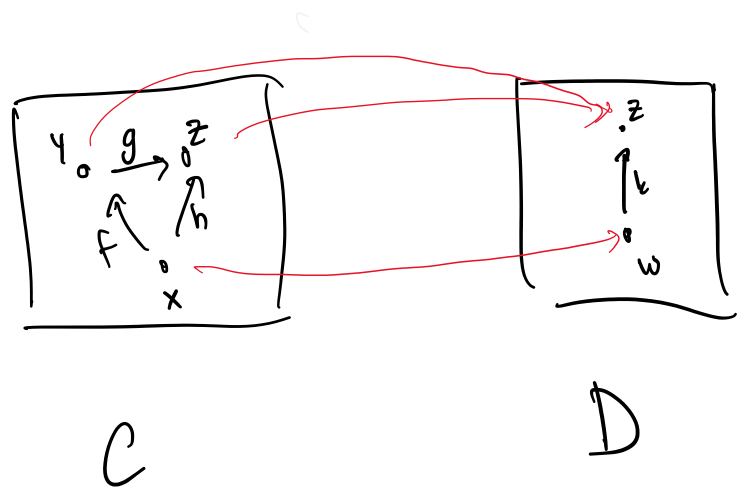
\includegraphics[width=0.5\linewidth]{fig/func-2.png}
\end{center}

The functor $F : \calC \to \calD$ is drawn in red; 
we've only shown its actions on objects here. Written out, 
we have:
\begin{align*}
  F(Y) = Z, \quad F(X) = W, \quad F(Z) = Z
\end{align*}
This action on objects defines the action on morphisms. 
This isn't always the case; there may be more than one morphism 
between two objects in $\calC$ and $\calD$, in which case, there may 
be a choice on which morphisms to map to. But here, it is simple,
and we can conclude:
\begin{align*}
  F(\id_Y) = \id_Z \quad F(\id_X) = \id_Z \quad F(\id_Z) = \id_Z \\
  F(g) = \id_Z \quad F(f) = k \quad F(h) = k
  \quad F(g \circ f) = k
\end{align*}

We need to check that the functoriality properties are 
satisfied. Clearly, identity preservation is satisfied. The only interesting 
case to check is the compositional property that $k = F(g \circ f) = F(g) \circ F(f) = \id_Z \circ k = k$.

As usual, it's useful to gain an intuition for what functors look like 
between categories that represent preorders. They will correspond to 
monotone functions:

\begin{definition}[Monotone function]
  Let $(X, \le_X)$ and $(Y, \le_Y)$ be preorders. Then, a 
  function $f : X \to Y$ is called \emph{monotone} if, 
  for any $x_1, x_2 \in X$ such that $x_1 \le_X x_2$, 
  it is the case that $f(x_1) \le_Y f(x_2)$.
\end{definition}

Now, let's see how functors between preorders correspond to monotone 
functions. 
Let $\calC$ and $\calD$ be categories corresponding to preorders
and let $F : \calC \Rightarrow \calD$ be a functor between 
these two categories.
Then, functoriality of $F$ requires that,
for any morphism $X \xrightarrow{f} Y$ in $\calC$, 
there is a morphism $F(X) \xrightarrow{f} F(Y)$.
This is exactly the monotonicity requirement:
the morphism $f$, considered order-theoretically, 
denotes that $X \le Y$; similarly, the morphism $F(f)$ 
denotes that $F(X) \le F(Y)$.



% Examples:
% \begin{itemize}
% \item Functors between two preorders are montone functions
% \item Denotational semantics of STLC is a functor \(\mathsf{STLC} \to \FinSet\)
% \item You may wonder: is a \(\calC\)-indexed set a functor? Hold that thought
% \end{itemize}


\section{Natural transformations}
Natural transformations are structure-preserving maps between functors:

\begin{definition}[Natural transformation]
  \sloppy
  Given two categories \(\calC\) and \(\calD\),
  and two functors \(F,G : \calC \to \calD\),
  a \emph{natural transformation \(\alpha\) from \(F\) to \(G\)},
  written
  \(\alpha : F \Rightarrow G\),
  consists of a function sending each object \(X\) of \(\calC\) to a \emph{morphism} \(F(X) \mor{\alpha_X} G(X)\) of \(\calD\)
  such that the following \emph{naturality condition} is satisfied:
  for each morphism \(X \mor{f} Y\) of \(\calC\), the following square commutes:
  \[
  % https://tikzcd.yichuanshen.de/#N4Igdg9gJgpgziAXAbVABwnAlgFyxMJZABgBpiBdUkANwEMAbAVxiRADEANEAX1PUy58hFGQCMVWoxZt2ATV78QGbHgJEx5SfWatEIAOLc+A1cI2kJ1HTP0GFPSTCgBzeEVAAzAE4QAtkhkIDgQSJpSurKeINQMdABGMAwACoJqIiDeWC4AFjiKXr4BiOEhSADM1tJ6IAA6tYxoOXQA+gqxCUmpZur6Wbn5JiA+-kgATNRliJURtobRQyPFQVMTszX1jc0txhQ8QA
\begin{tikzcd}
FX \arrow[d, "Ff"'] \arrow[r, "\alpha_X"] & GX \arrow[d, "Gf"] \\
FY \arrow[r, "\alpha_Y"']                 & GY
\end{tikzcd}
  \]
  In other words, \(\alpha_Y \circ Ff = Gf \circ \alpha_X\) for all \(X \mor{f} Y\).
\end{definition}

Let's consider two functors $F$ and $G$ between finite categories and a 
natural transformation $\alpha : F \Rightarrow G$:
\begin{center}
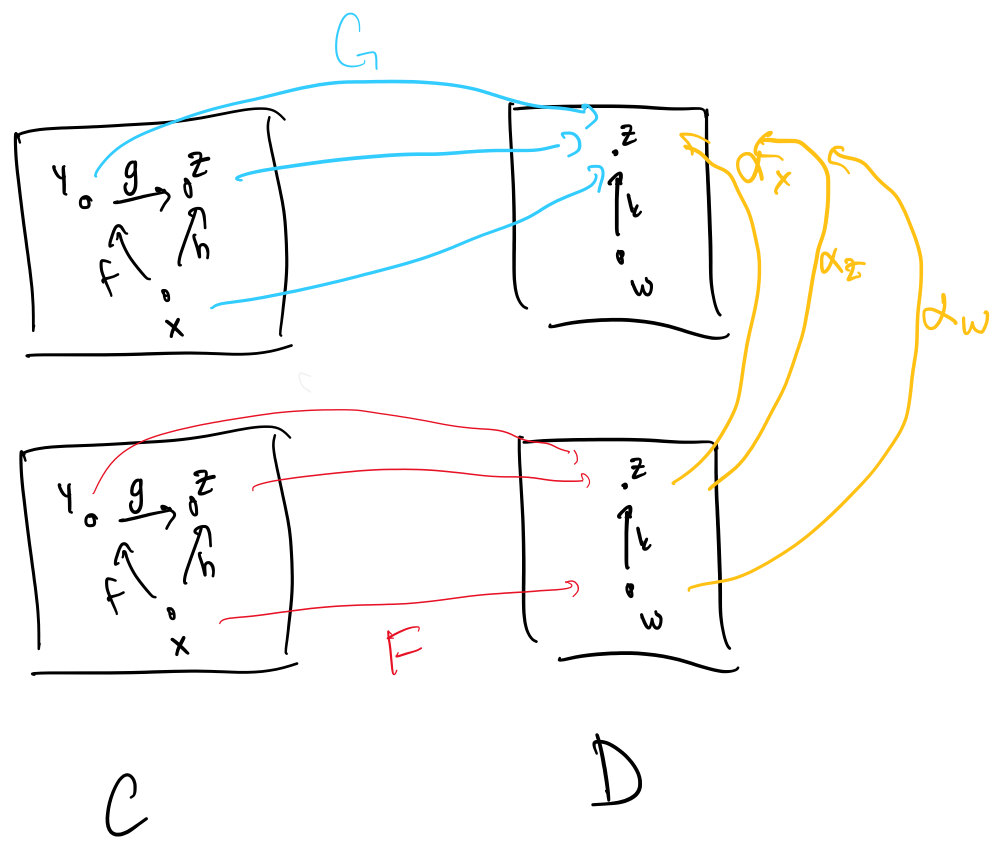
\includegraphics[width=0.8\linewidth]{fig/nat-trans1.png}
\end{center}

Breaking the data in this figure down, we have that $\alpha_X = \id_Z$, 
$\alpha_Z = \id_Z$, and $\alpha_W = k$. Now we can 
check the naturality square for every morphism:
\begin{itemize}
  \item Checking for $f$: we need to show that $\alpha_Y \circ F(f) = G(f) \circ \alpha_X$.
  Substituting, this is $\id_Z \circ k = \id_Z \circ k$.
\end{itemize}


\subsection{More examples of natural transformations}

Think back to \(\calC\)-indexed functions. We drew these as squares involving two Balloon diagrams stacked together.
It may help to think of the naturality condition as an abstraction of such a picture, where Balloons are replaced by
objects of \(\calD\):
\[% https://tikzcd.yichuanshen.de/#N4Igdg9gJgpgziAXAbVABwnAlgFyxMJZABgBoBmAXVJADcBDAGwFcYkQANEAX1PU1z5CKAIwVqdJq3YBNHnxAZseAkTIiJDFm0QgAYl179lQtaWKapOkAHFDCpYNWjSGmlum69co4oErhZDELdyt2Gx8JGCgAc3giUAAzACcIAFskMhAcCCQxSW12RPkk1IzEACYaHKQAFlDCr2KaRnoAIxhGAAV-U11krBiACxwSkBT0pHJq3MQAVgbPW2LfCfKq7NnpgqWAHV2mNCH6AH17UsnEes2kBZ3rfcPjk4BPEBb2zp6TZxAB4dG3Eo3CAA
\begin{tikzcd}
GX \arrow[r, "Gf"]                        & GY                        \\
FX \arrow[r, "Ff"'] \arrow[u, "\alpha_X"] & FY \arrow[u, "\alpha_y"'] \\
                                          &                           \\
X \arrow[r, "f"]                          & Y
\end{tikzcd}\]

\begin{definition}[Identity natural transformation]
  Let \(F : \calC \to \calD\) be a functor between two categories \(\calC,\calD\).
  The identity natural transformation \(\idt_F : F \Rightarrow F\)
  is defined by \(\idt_{F,X} = \idt_{F(X)}\).
  Naturality is verified by the following ``abstract balloon diagram'':
  \[% https://tikzcd.yichuanshen.de/#N4Igdg9gJgpgziAXAbVABwnAlgFyxMJZABgBoBmAXVJADcBDAGwFcYkQANEAX1PU1z5CKAIwVqdJq3YBNHnxAZseAkTIiJDFm0QgAYl179lQomI00t03XrlHFAlcJKlimqTv2GFSwatGu7trstjwSMFAA5vBEoABmAE4QALZIZCA4EEhiksG6cfLxSamIACw0mUgArJYeIQX2iSlIAEwVWYjktXn6DQpNJW0ZHeW51iAAOhNYUDgA+sAG3IUgA0hdw9Xd41Mz84syy9yU3EA
\begin{tikzcd}
FX \arrow[r, "Ff"]                        & FY                        \\
FX \arrow[r, "Ff"] \arrow[u, "\idt_{FX}"] & FY \arrow[u, "\idt_{FY}"] \\
                                          &                           \\
X \arrow[r, "f"]                          & Y
\end{tikzcd}\]
\end{definition}

\begin{definition}[Composition of natural transformations]
  Given \(\alpha : F \Rightarrow G\) and \(\beta : G \Rightarrow H\),
  the composition \(\beta\circ \alpha : F \Rightarrow H\) is defined by
  \((\beta\circ\alpha)_{X} = \beta_X \circ \alpha_X\).
  Naturality is verified by the following ``abstract balloon diagram'':
  \[% https://tikzcd.yichuanshen.de/#N4Igdg9gJgpgziAXAbVABwnAlgFyxMJZABgBoAWAXVJADcBDAGwFcYkQANEAX1PU1z5CKAIwVqdJq3YBNHnxAZseAkTIAmCQxZtEIAGJde-ZUKJjNNbdL365xxQJXCSpEVqm6QAcSMKlgqqibh467N72-k5mKGTEoTYgABJ+JoEuYvFWnuxJ9hIwUADm8ESgAGYAThAAtkhkIDgQSGKSYXrl8hXVdYjkNE1IAKzZ7T6dDlW1SOoDzYgAzKOJ+hMKU72zjfP9bYkAOvtMaAAW9AD6qSAbSEvbw8teh8dn53I0jPQARjCMAArRIIgSpYIonHBda49JC7QaIABsj3Yhx+OAuVxuiBG90QAHYkXoUTA0W8QB9vr8AaYgSCwRDJtCEXMkPi9l4khNKNwgA
\begin{tikzcd}
HX \arrow[r, "Hf"]                       & HY                        \\
GX \arrow[r, "Gf"] \arrow[u, "\beta_X"]  & GY \arrow[u, "\beta_Y"']  \\
FX \arrow[r, "Ff"] \arrow[u, "\alpha_X"] & FY \arrow[u, "\alpha_Y"'] \\
                                         &                           \\
X \arrow[r, "f"]                         & Y
\end{tikzcd}\]
\end{definition}

Examples
\begin{itemize}
\item Suppose you have two functors \(F,G : X \to Y\) between preorders \(X,Y\), aka two monotone functions.
  There is at most one natural transformation \(\alpha : F \Rightarrow G\), which exists if and only if \(F(x) \le G(x)\) for all \(x\in X\).

\item Mind-bending example: there is an identity functor \(\mathsf{id} : \FinSet \to \FinSet\).
  What does a natural transformation \(\alpha : \mathsf{id} \Rightarrow \mathsf{id}\) look like?
  Think polymorphism: intuitively, \(\alpha\) must have type ``\(\forall X. \FinSet(\mathsf{id}(X),\mathsf{id}(X))\)'',
  aka ``\(\forall X. X \to X\)''.
  This suggests that \(\alpha\) is the identity, i.e., \(\alpha_X = \idt_X\) for all objects \(X\) of \(\FinSet\).
  Indeed, we can verify this follows from \(\alpha\) being natural, as follows.
  \begin{itemize}
  \item Let \(X\) be an arbitrary object of \(\FinSet\). We will show \(\alpha_X\) is the identity function on \(X\).
  \item By function extensionality it's enough to show that for all \(x \in X\) it holds that \(\alpha_X(x) = x\).
  \item Fix \(x \in X\) arbitrary. We saw in a homework that \(x\) corresponds to a \(\FinSet\) morphism \(\hat x : 1 \to X\),
    where \(1\) is the terminal object of \(\FinSet\) (aka the one-point set).
    Now, by naturality of \(\alpha\), the following square commutes:
    \[% https://tikzcd.yichuanshen.de/#N4Igdg9gJgpgziAXAbVABwnAlgFyxMJZABgBoBGAXVJADcBDAGwFcYkRyQBfU9TXfIRTkK1Ok1btOPPtjwEiZYmIYs2iEAA1uvEBjmCiI5TVWSN2rmJhQA5vCKgAZgCcIAWyRkQOCEhHiauwAOsFMaAAW9AD6nDSM9ABGMIwACvzyQiAuWLYRODrObp6I3r5IAEymEuogAB6FIK4e-jTliADM1UEaDfFJKekGCho5eQUyTcWVbX6d3eYgoeFR0ZaUXEA
\begin{tikzcd}
X \arrow[r, "\alpha_X"]                 & X                 \\
1 \arrow[r, "\alpha_1"'] \arrow[u, "x"] & 1 \arrow[u, "x"']
\end{tikzcd}\]
    Because \(1\) is terminal, there can only be one morphism \(1\to 1\), namely the identity. Hence \(\alpha_1 = \idt_1\).
    Thus this square collapses to the following triangle:
    \[% https://tikzcd.yichuanshen.de/#N4Igdg9gJgpgziAXAbVABwnAlgFyxMJZABgBoBGAXVJADcBDAGwFcYkRyQBfU9TXfIRRli1Ok1bsAGt14gM2PASLlSomgxZtEIGVzEwoAc3hFQAMwBOEALZIyIHBCSrxW9gA9ZF63cSunJAAmDQltEAAdCKY0AAt6AH09OStbexpAxBC3SR0vGkZ6ACMYRgAFfiUhEEssI1icbkouIA
\begin{tikzcd}
X \arrow[r, "\alpha_X"]           & X \\
1 \arrow[u, "x"] \arrow[ru, "x"'] &
\end{tikzcd}\]
But now this triangle expresses the fact that \(\alpha_X(x) = x\), which is exactly what was to be shown.
  \end{itemize}
\end{itemize}

\section{Functor categories}

\begin{definition}[Functor category]
  Let \(\calC\) and \(\calD\) be categories.
  Suppose that
  \begin{enumerate}
    \item The collection of functors from \(\calC\) to \(\calD\) forms a set
    \item For any two functors \(F,G : \calC \to \calD\), the collection of natural transformations from \(F\) to \(G\) forms a set
  \end{enumerate}
  Then there is a \emph{functor category}, written \([F;G]\), whose
  \begin{itemize}
  \item Objects are functors \(\calC\) to \(\calD\)
  \item Morphisms from \(F\) to \(G\) are natural transformations \(\alpha : F \Rightarrow G\)
  \end{itemize}
  Identity morphism is the identity natural transformation, and composition is composition of natural transformations.
\end{definition}

Examples
\begin{itemize}
\item As you can see, there are small set-theoretic nuisances with this definition. We will come back to this
\item \(\FinSet^{\mathsf{loop}}\) is a functor category! It's the functor category \([\calC;\FinSet]\) where \(\calC\) is the
  category with one object \(\star\), a special non-identity morphism \(f\), and all composites one can make from this (aka \(f^n\) for \(n\in \N\)).
  (In other words, \(\calC\) is the category you get from the monoid \((\N,+,0)\) of natural numbers under addition.)
\item \(\FinSet^{\bullet\to\bullet}\), the category of finite functions, is a functor category! It's \([(\bullet \to\bullet); \FinSet]\)
  where \(\bullet\to\bullet\) is the category with two objects and one non-identity arrow between them.
\item As you can see, functor categories are kind of like ``categories of diagrams'': the objects of a functor category look like
  diagrams whose shape is given by the domain category. Keep this in mind; it'll come back later (limits and colimits)
\item You may wonder: are \(\calC\)-indexed sets a functor category? Hold that thought...
\end{itemize}

\section{Full and faithful functors}
We noted that a functor $F : \calC \to \calD$ ensures an abstract copy of 
$\calC$ is inside $\calD$. But, what if we want \emph{more} of $\calC$ 
to be visible inside $\calC$? We can coax more structure out by 
enforcing that the functor does not collapse any structure.

Note that for each functor \(F : \calC \to \calD\) and each pair of objects \(X,Y\) in \(\calC\),
you get a function \(\calC(X,Y) \to \calD(FX,FY)\).
\begin{itemize}
\item A functor is \emph{full} if this function is surjective: for any morphism \(FX \mor{\hat f} FY\) in \(\calD\),
  there exists a morphism \(X \mor{f} Y\) in \(\calC\) such that \(\hat f = F(f)\).
\item A functor is \emph{faithful} if this function is injective: for any morphism for any morphisms \(f,g : X \to Y\) in \(\calC\),
  if \(Ff = Fg\) as morphisms \(FX\to FY\) in \(\calD\), then \(f = g\).
\end{itemize}
In particular, if a functor is \emph{full and faithful}, then each function \(\calC(X,Y) \to \calD(FX,FY)\) is a bijection,
showing that \(\calD(FX,FY) \cong \calC(X,Y)\) for all objects \(X,Y\) of \(\calC\).



\section{The category of sets}

Naive definition, paralleling \Cref{def:finset}: the category \(\Set\) consists of
\begin{itemize}
\item Objects: the set of all sets
\item Morphisms: tuples \((A,f,B)\) where \(A,B\) are sets and \(f : A \to B\) is a function
\end{itemize}
Obviously this definition is unworkable: there is no set of all sets.
We have to finally confront the set-theoretic minutiae that we have swept under the rug so far.
Russell famously showed that the collection of all sets does not form a set; it is ``too big''.
We will adopt a way out which has become standard when doing highly categorical things:
postulate the existence of a ``very big set'' that contains ``enough sets to look like the set of all sets''.
\begin{definition}[Grothendieck universe]
  A Grothendieck universe is a set \(U\) satisfying the following properties:
  \begin{itemize}
    \item Copy from Definition 2.1 of \href{https://ncatlab.org/nlab/show/Grothendieck+universe}{the nLab page}
  \end{itemize}
\end{definition}
Every Grothendieck universe \(\calU\) is a model of ZFC, hence ``looks like the set of all sets''.
From now on we assume the following axiom.
\begin{axiom}
  There exists a Grothendieck universe \(\calU\).
\end{axiom}
The set \(\calU\) splits the world of sets into two halves:
\begin{itemize}
\item On one side there are the sets \(X\) such that \(X \in \calU\). These sets are ``small enough to fit into \(\calU\)'', so called \emph{\(\calU\)-small}.
\item On the other side there aer sets \(X\) such that \(X \notin \calU\). these sets are ``too large to fit'', so called \emph{\(\calU\)-large}.
\end{itemize}

The key point is that, we cannot define a category of \emph{all} sets, we  can define a category of \emph{\(\calU\)-small} ones.
\begin{definition}[the category of (\(\calU\)-small) sets]
  \(\Set\) is the category whose
  \begin{itemize}
    \item Objects are elements of \(\calU\), aka \(\calU\)-small sets
    \item Morphisms from \(X\) to \(Y\) are functions \(f : X \to Y\)
  \end{itemize}
\end{definition}
Just as sets can be \(\calU\)-small or \(\calU\)-large, so too can categories.
There are actually three tiers of ``small''-ness for categories.
First, a category can fit perfectly inside of the universe \(\calU\).
\begin{definition}
  A category \(\calC\) is \emph{\(\calU\)-small} if both of its sets of objects and morphisms are.
\end{definition}
More generally, a category could be too large to fit inside of \(\calU\), but it could be the case that for any two objects,
the collection of \emph{morphisms} between those two objects does fit inside of \(\calU\).
Intuitively, this is like saying the category is \(\calU\)-small if you zoom in on the morphisms betwen two given objects;
hence this condition is called being ``locally'' small.
\begin{definition}
  A category \(\calC\) is \emph{\(\calU\)-locally-small} if, for each pair of objects \(X,Y\),
  the set \(\calC(X,Y)\) is \(\calU\)-small.
\end{definition}
Finally, a category is \(\calU\)-large if it is neither small nor locally small.

\subsection{Indexed set theory as a category}
Now we can show that \(\calC\)-indexed sets form a category.
\begin{definition}[category of \(\calC\)-indexed sets]
  Let \(\calC\) be a locally \(\calU\)-small category.
  Then \(\calC\)-indexed sets and functions between them form a functor category \([\calC^{\mathsf{op}};\Set]\).
\end{definition}

\begin{proposition}
  Let \(\calC\) be a locally \(\calU\)-small category.
  The Yoneda embedding defines a functor \(\yo : \calC \to [\calC^{\mathsf{op}};\Set]\),
  and this functor is full and faithful.
\end{proposition}
\begin{proof}
  Let $X$ and $Y$ be objects. To show that $\yo$ is full and faithful,
  we must show that $\calC(X, Y) \cong [\calC^{\mathsf{op}}; \Set](\yo X, \yo Y)$.

  Let $X$ and $Y$ be objects.
  Then, 
  by specializing the baby Yoneda lemma,
  $\{\alpha : \yo X \Rightarrow \yo Y\} \cong \yo(Y)(X)$. 
  We have immediately that $\{\alpha : \yo X \Rightarrow \yo Y\} = [\calC^{\mathsf{op}}; \Set](\yo X, \yo Y)$ 
  by the definition of a functor category,
  and that $\yo(Y)(X) = \calC(X, Y)$ by the 
  definition of $\yo$.
  \end{proof}

%% \subsection{The Yoneda lemma in full generality}

%% We finally have enough language to state the non-baby version of the Yoneda lemma.
%% \begin{definition}
%%   Let \(\calC\) be a \(\calU\)-locally small category.
%%   Then
%%   \[
%%     [\calC^{\mathsf{op}}](\yo X, F) \cong F(X)
%%   \]
%%   natural in \(F,X\),
%%   which means that there is a natural isomorphism between two functors
%%   \[% https://tikzcd.yichuanshen.de/#N4Igdg9gJgpgziAXAbVABwnAlgFyxMJZABgBpiBdUkANwEMAbAVxiRGQB0OBjRgYQB6wLgFs6OABZwAZsAhoAvgoDcXAMowcFAARc8I+Lp78ho8VNnylIBaXSZc+QigBM5KrUYs26zTY8wUADm8ESg0gBOECJIZCA4EEgAjNQARjBgUEgAtADMcfTMrIggejAAHjjAAEoAEmoKINQMdOkMAAoOeARsEVhBEjg2diCR0bHUCclpGVmI+dSF3iVllcAAMvWNChQKQA
%% \begin{tikzcd}
%% {[\calC^{\mathsf{op}};\Set] \times \calC^{\mathsf{op}}} \arrow[rr, "\text{RHS}"', bend right] \arrow[rr, "\text{LHS}", bend left] &  & \Set
%% \end{tikzcd}\]
%% where \(\text{LHS}\) is the functor defined by
%% \begin{itemize}
%% \item On objects, \(\text{LHS}(F,X) = [\calC^{\mathsf{op}}](\yo X, F)\)
%% \item On morphisms \(\), \(\text{LHS}(F,X) = [\calC^{\mathsf{op}}](\yo X, F)\)
%% \end{itemize}
%% \end{definition}


%% - Grothendieck universes
%% - The category Set
%% - Functors; opposite categories; C-indexed sets as functors
%% - Natural transformations; C-indexed functions as natural transformations
%% - The Yoneda lemma (without showing naturality in P,c)

%% \begin{itemize}
%% \item Functors form a category where morphisms are natural transformations \begin{itemize}
%%     \item Natural transformations as homotopies between diagrams
%%       (the \(C\to D^\to\) example revisited)
%%     \item Natural transformations as polymorphic maps
%%   \end{itemize}
%% \item Definition of Yoneda embedding
%% \item Restatement of universal properties from previous week in terms of Yoneda embedding
%% (e.g., for products, \(\yo(a\times b) \cong \yo(a)\times \yo(b)\).)
%% \item Yoneda embedding full and faithful. Use this to quickly prove some basic facts:
%%   associativity and commutativity of sums and products, distributivity of products over sums,
%%   ...
%%   These imply type isomorphisms in STLC and Set, entailments of propositional logic.
%% \item Yoneda preserves limits.
%%   This gives a quick proof that all limits can be constructed from products and equalizers.
%%   From this we can compute limits in STLC (it won't have all of them
%%   but it will have some).
%% \end{itemize}

%% \todo: \begin{itemize}
%% \item Slice over c is category of elements of yo c
%% \end{itemize}
